\chapter{Desarrollo de la Aplicación}\label{chapter:Desarrollo de la Aplicacion}

Este capítulo describe las actividades realizadas en la concepción, diseño, construcción y transición del prototipo de la aplicación web y de la aplicación móvil de Notificaciones+. 
Está dividido en secciones, cada una de ellas representando una fase de la metodología adoptada, descrita en el capítulo anterior.

\section{Concepción} \label{sect:Concepcion}
El objetivo de esta fase consistió en recolectar la información necesaria para levantar los requerimientos del cliente para las aplicaciones a desarrollar. Por este motivo se realizaron reuniones periódicas con el mismo para determinar detalladamente dichos requerimientos y definir las características que tanto la aplicación web, como la aplicación móvil de Notificaciones+ debería poseer.
Esta fase tuvo una duración de 2 semanas, y se realizaron las siguientes actividades:
\smallskip
\begin{itemize}[noitemsep,nolistsep]
  \item Familiarización con la empresa y el entorno laboral.
  \item Investigación sobre las prácticas de la empresa.
  \item Levantamiento de requerimientos funcionales y no funcionales.
  \item Identificación y mitigación de riesgos que puedan afectar el desarrollo del sistema.
  \item Investigación general de herramientas disponibles para ambas aplicaciones (Web y Móvil)
  \item Investiagación de la plataforma Synergy Push.
\end{itemize}
\bigskip

En esta etapa del desarrollo, se inició el documento de especificación funcional y el documento de Arquitectura de Software de Notificaciones+ para Synergy-GB, el cual se refinó en repetidas oportunidades de acuerdo a las solicitudes que el cliente realizó (ver Apéndice B, el cual incluye los requerimientos).

\subsection{Requerimientos}
La lista de requerimientos se realizó de acuerdo al plan de trabajo y a varias reuniones con el cliente para aclarar todo el objetivo de ambas aplicaciones. En la Tabla ~\ref{table:ReqFunc} se presenta un resumen de los requerimientos funcionales de la aplicación web y de la aplicación móvil de Notificaciones+ (véase el Apéndice B para más información).

\begin{table}[H]
%\centering 
\begin{tabular}{| p{6cm} | p{10cm} |}
\hline 
\bfseries \footnotesize {Requerimiento} & \bfseries \footnotesize {Descripción} \\ 
\hline 
\bfseries 
  \footnotesize {Gestionar sesión} &
  \footnotesize Un usuario debe poder iniciar sesión luego de autenticar sus credenciales y cerrar una sesión previamente iniciada. \\ \hline 
\bfseries 
  \footnotesize {Permitir registro} & 
  \footnotesize Un usuario debe poder registrarse desde su dispositivo móvil a la plataforma Synergy Push Services para poder luego iniciar sesión y usar la plataforma. \\ \hline 
\bfseries 
  \footnotesize {Recibir Notificación Push} & 
  \footnotesize El dispositivo del usuario debe poder recibir automáticamente notificaciones Push provenientes de la plataforma Synergy Push Services, una vez el usuario haya iniciado sesión. \\ \hline 
\bfseries \footnotesize {Recibir y Abrir Mensajes Completos} & \footnotesize Un usuario debe poder seleccionar una notificación de su buzón y abrirla para ver todo su contenido. \\ \hline 
\bfseries 
  \footnotesize {Devolver respuesta de una o dos opciones a mensajes que lo requieran} & 
  \footnotesize Un usuario debe poder seleccionar una opción de respuesta a mensajes que requieran esta acción por parte del usuario, como alertas de seguridad interactiva y notificaciones de operaciones bancarias. \\ \hline 
\bfseries 
  \footnotesize {Compartir Mensaje} & 
  \footnotesize Un usuario debe poder compartir desde el buzón y la vista de detalles, un mensaje a través de otras aplicaciones instaladas en su dispositivo móvil. \\ \hline 
\bfseries 
  \footnotesize {Eliminar Mensajes} & 
  \footnotesize Un usuario debe poder eliminar desde el buzón y la vista de detalles, cualquier mensaje que se encuentre allí. \\ \hline 
\end{tabular}
\footnotesize \caption{Resumen de requerimientos funcionales de la aplicación web y de la aplicación móvil de Notificaciones+. Elaboración propia.}
\label{table:ReqFunc}
\end{table}

Un resumen de los requerimientos no funcionales pueden verse en la Tabla ~\ref{table:ReqNoFunc} (pueden consultarse a detalle en el Apéndice B).

\begin{table}[H]
\centering 
\begin{tabular}{| p{3cm} | p{13cm} |}
\hline 
\bfseries \footnotesize {Requerimiento} & \bfseries \footnotesize {Descripción} \\ 
\hline 
\bfseries \footnotesize {Funcionalidad} & \footnotesize El sistema debe cumplir con todas las funcionalidades especificadas en los casos de uso. \\ \hline 
\bfseries \footnotesize {Usabilidad} & \footnotesize El sistema debe ser fácil e intuitivo de usar.  \\ \hline 
\bfseries \footnotesize {Eficiencia} & \footnotesize El sistema debe llevar a cabo todos sus procesos de manera rápida y eficiente.  \\ \hline 
\end{tabular}
\footnotesize \caption{Resumen de requerimientos no funcionales de la aplicación web y de la aplicación móvil de Notificaciones+. Elaboración propia.}
\label{table:ReqNoFunc}
\end{table}


% En la Figura ~\ref{fig:arqbb+} se muestra la especificación del requerimiento “Consultar beneficiarios”, incluyendo las interfaces y estructuras de datos asociadas. En el Apéndice B se encuentra la especificación para cada uno de los requerimientos de la Tabla ~\ref{table:ReqNoFunc} y la Tabla ~\ref{table:ReqFunc}.
% \begin{figure}[ht]
%   \centering
%   \includegraphics[scale=1,type=png,ext=.png,read=.png,angle=0,origin=c]{imagenes/reqespec}
%   \caption{Especificación del Requerimiento Consultar Directorio. Elaboración propia.}
%   \label{fig:arqbb+}
% \end{figure}


\subsection{Riesgos}
El propósito de la lista de riesgos es, en primer lugar, identificar aquellos elementos que pueden afectar negativamente la ejecución del proyecto. Además, permite medir el impacto de cada riesgo y planificar estrategias de mitigación y acciones de contingencia en caso de materializarse alguno de ellos.


Los principales riesgos detectados fueron, en su mayoría, desacuerdos que se originaban por problemas de comunicación entre el desarrollador y el cliente, además de desiciones de diseño que no estaban tomadas y quedaban a improvisación por parte del desarrollador. No obstante, como en este caso el rol de cliente es asumido por la misma empresa Synergy-GB,  las acciones tomadas para mitigar estos riesgos consisten en la realización de reuniones periódicas para mantener los objetivos y requerimientos claros y actualizados.


Probablemente el mayor riesgo sea que la funcionalidad principal de la aplicación, que son la recepción de notificaciones Push, dependían de \textit{software} de terceros, experimental, ajeno a la plataforma Ionic, del cual la compañía nunca había utilizado y no había ninguna garantía que funcionara. 


Otros riesgos que influían en el desarrollo de la aplicación fueron aquellos asociados al cálculo erróneo del tiempo de desarrollo, la pendiente de la curva de aprendizaje de determinadas herramientas utilizadas para el desarrollo del proyecto, en especial AngularJS y su interacción con Cordova, y la subestimación del monto de esfuerzo a ser empleado. Todos estos riesgos fueron mitigados con estrategias de planificación que contemplaran la importancia de los componentes críticos de la aplicación y la complejidad de ciertas herramientas a utilizar.


\subsection{Tecnologías y plataformas de desarrollo}
El proyecto tenía que ser desarrollado bajo ambientes adecuados y hacer uso de tecnologías innovadoras que otorgaran el máximo de beneficios. Para la implementación de la aplicación móvil de Notificaciones+ se utilizaron las herramientas implícitas (frameworks, lenguajes y plataformas) en el desarrollo de una aplicación multiplataforma con Ionic Framework. En orden piramidal: 
\smallskip
\begin{itemize}[noitemsep,nolistsep]
  \item Ionic Framework
  \item AngularJS
  \item JavaScript
  \item HTML5/CSS3
  \item ngCordova
  \item Cordova/Phonegap
  \item iOS/Android
\end{itemize}
\bigskip

Se usó Sublime como editor de texto. Toda la programación se hizo en una PC corriendo Ubuntu 14.10. Se usó un computador MAC OSX para compilar y correr bajo la plataforma iOS debido a las políticas de exclusividad de esa herramienta. También se hizo uso limitado de los respectivos emuladores Android y iOS. Los dispositivos de prueba fueron:
\smallskip
\begin{itemize}[noitemsep,nolistsep]
  \item iPhone 5 con iOS 7
  \item Samsung Galaxy Nexus con Android 4.3 
  \item HTC One S con Android 4.1.1
  \item Huawei con Android 4.4
\end{itemize}
\bigskip 


\subsection{Casos de Uso}

Los Casos de Uso proporcionan uno o más escenarios, los cuales definen la secuencia acciones que debe llevar a cabo el usuario para activar una funcionalidad de las aplicaciones.

El Modelo de Casos de Uso de la aplicación es utilizado con el fin de ilustrar tanto las funcionalidades como la relación entre ellas y los actores que las usan. En la Figura ~\ref{fig:dcuinicial} se puede observar el Diagrama de Casos de Uso inicial, que posteriormente se refinó ya que se ampliaron las funcionaliades y se aclararon ciertos requerimientos de \textit{software}.

En el mismo se observa que se identificaron dos actores. En primer lugar, el Usuario, que se encarga de hacer uso de Notificacones+. Luego, el otro actor es Synergy Push que es la plataforma a la cual se conecta la aplicación para obtener mensajes.


\subsection{Planificación Inicial}

Esta actividad consistió en estimar una planificación para el desarrollo del proyecto: el orden en que serán implementados los Casos de Uso (CU) y el tiempo que debía tomar cada uno de ellos. La Figura ~\ref{fig:dcuinicial} muestra el diagrama de Casos de Uso Inicial que permitío establecer la planificación. 

\begin{figure}[ht]
  \centering
  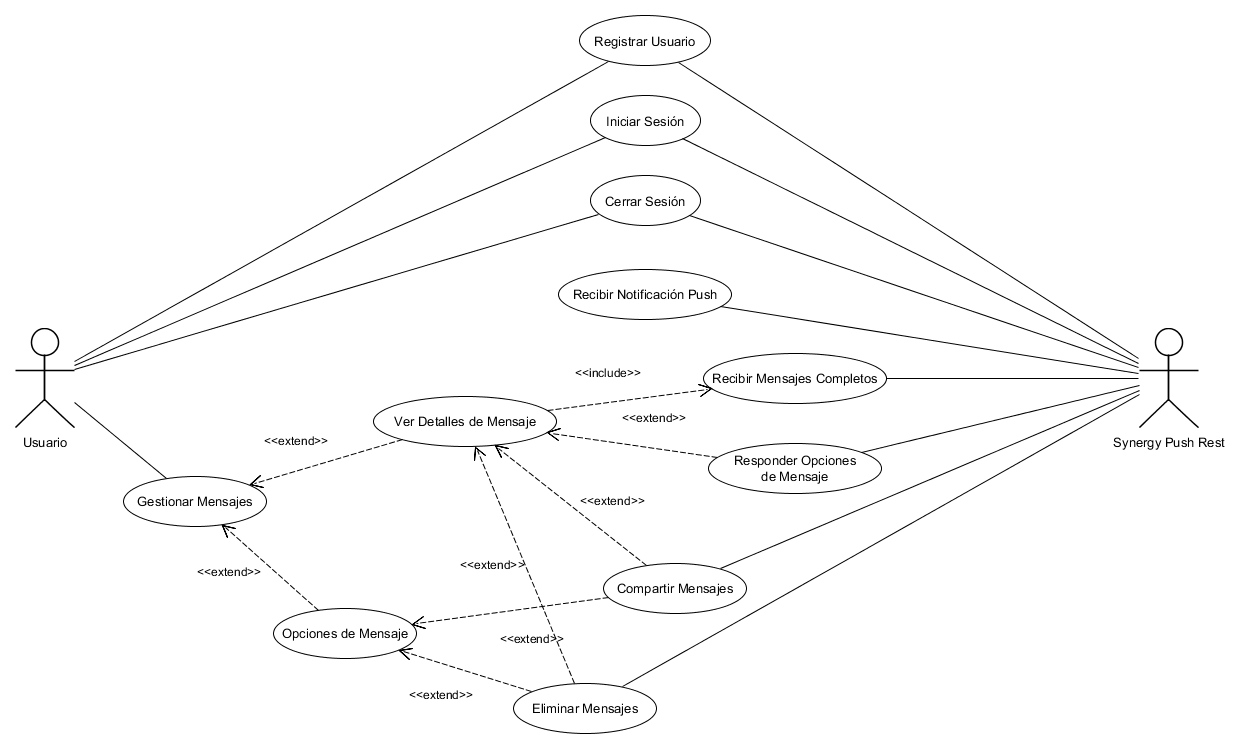
\includegraphics[scale=0.3,type=png,ext=.png,read=.png,angle=0,origin=c]{imagenes/Diagrama_de_Casos_de_Uso_v1_5}
  \caption{Diagrama de Casos de Uso inicial de Notificacones+. Elaboración propia.}
  \label{fig:dcuinicial}
\end{figure}


Luego, se estableció un plan de cuatro iteraciones de 4 semanas cada una, aproximadamente. En la primera iteración se planificó hacer todas las vistas tanto su diseño como su implementción en Ionic con HTML5/CSS3. En a segunda iteración se planificó llevar a cabo los CU relacionados con “Gestionar Mensajes”. En la tercera iteración los CU relacionados con “Recibir Notificaciones Push”, “Registrarse” y “Recibir Mensajes Completos” que son las involcradas directamente con plataforma Synergy Plus.  Finalmente, en la última iteración los CU que permitan iniciar y cerrar sesión y todos los demás detalles que falten.


\section{Diseño} \label{sect:Diseno}
En esta fase, inicialmente se estudiaron los requerimientos del dueño del producto y el API REST de Synergy Plus, para así elaborar las maquetas visuales de la aplicación siguiendo los lineamientos establecidos para el desarrollo de \textit{software} de la empresa. Luego se pasó a hacer una elaboración de las vistas basadas en las maquetas mientras éstas eran aprobadas por el dueño del producto y fuera elaborado el diseño definitivo por parte del departamento de diseño. 


\subsection{Diseño de la arquitectura}
A la hora de diseñar la arquitectura de este sistema, se tuvo en consideración las siguientes importantes características:
\smallskip
\begin{itemize}[noitemsep,nolistsep]
  \item Escalabilidad: Debe poder instanciarse de manera fácil a cualquier banco (u otro cliente que necesite un producto como Notificaciones+), de manera que el producto sea rentable con una fácil personalización de acuerdo a lo que se solicite.
  \item Modularidad: Debe ser lo más modular y de bajo acoplamiento posible para evitar inconvenientes cuando se necesiten hacer cambios a la aplicación.
  \item Flexibilidad: Debe poder cambiar incluso su funcionalidad de la manera menos traumática posible.
\end{itemize}
\bigskip

\subsubsection{Vista de Escenarios}
En la Figura ~\ref{fig:cudef} se presenta el Diagrama de Casos Uso definitivo del proyecto de pasantía Notificaciones+ para Synergy-GB. Se puede ver como en el transcurrir de las iteraciones cambió el diagrama de acuerdo a nuevos requerimientos del cliente. Lo que es más pertinente de acotar es que los Casos de Uso son iguales tanto para la aplicación móvil como la aplicación web, exceptuando "Recibir Notificaciones Push" que es exclusivo de la aplicación móvil.

\begin{figure}[H]
  \centering
  
\includegraphics[scale=0.3,type=png,ext=.png,read=.png,angle=0,origin=c]{imagenes/Diagrama_de_Casos_de_Uso_v2_0}
  \caption{Diagrama de casos de uso definitivo de Notificaciones+. Elaboración propia.}
  \label{fig:cudef}
\end{figure}


En la Figura ~\ref{fig:cupush} se presenta la especificación del CU “Recibir Notificación Push”. En el Apéndice B se pueden consultar las especificaciones de todos los CU del diagrama de la Figura ~\ref{fig:cudef}.

\begin{figure}[ht]
  \centering
  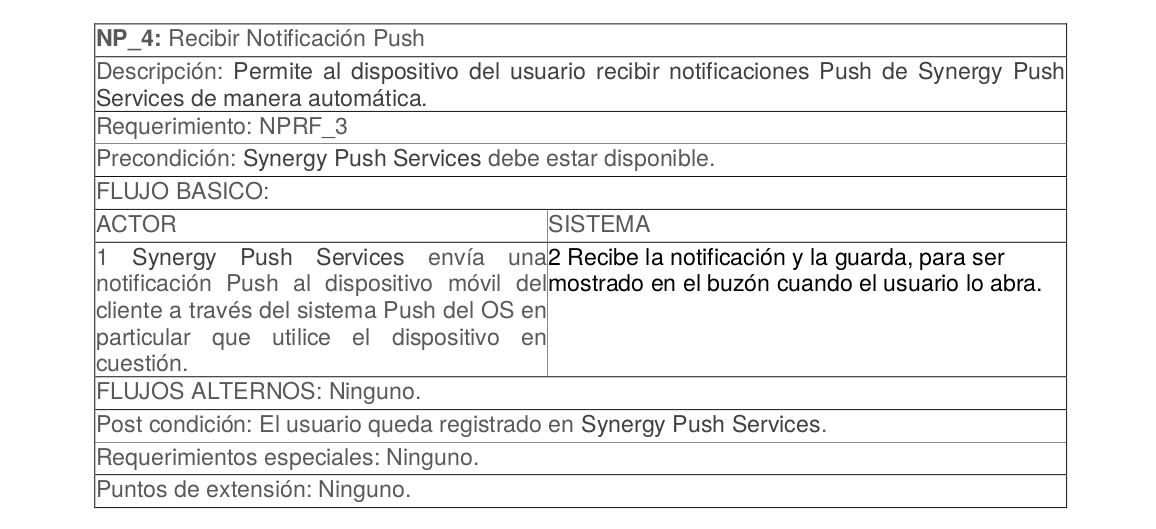
\includegraphics[scale=0.4,type=png,ext=.png,read=.png,angle=0,origin=c]{imagenes/cupush}
  \caption{Especificación del Caso de Uso “Recibir Notificación Push”. Elaboración propia.}
  \label{fig:cupush}
\end{figure}


\subsubsection{Vista Lógica}
Las aplicaciones (web y móvil) estarán conformadas por clases que se encargarán de definir los objetos que se manejan en el sistema y su relación. A continuación, en la Figura ~\ref{fig:clases} se muestra el Diagrama de Clases para Notificaciones+, el cual representa la Vista Lógica de la misma. 

\begin{figure}
  \centering
  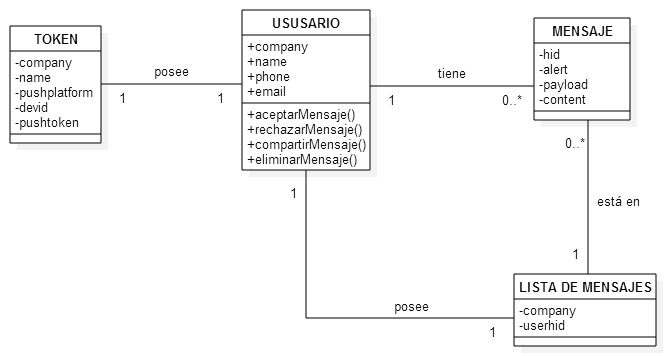
\includegraphics[scale=0.4,type=png,ext=.png,read=.png,angle=0,origin=c]{imagenes/Diagrama_de_Clases}
  \caption{Diagrama de Notificaciones+. Elaboración propia.}
  \label{fig:clases}
\end{figure}


En el diagrama de clases se pueden observar las estructuras manejadas por la plataforma Synergy Push y por lo tanto por la aplicación.


\subsubsection{Vista de Desarrollo}
La vista de desarrollo de la arquitectura de Notificaciones+ se ve reflejada en el Diagrama de Componentes que se muestra en la Figura ~\ref{fig:componentes}


\begin{figure}
  \centering
  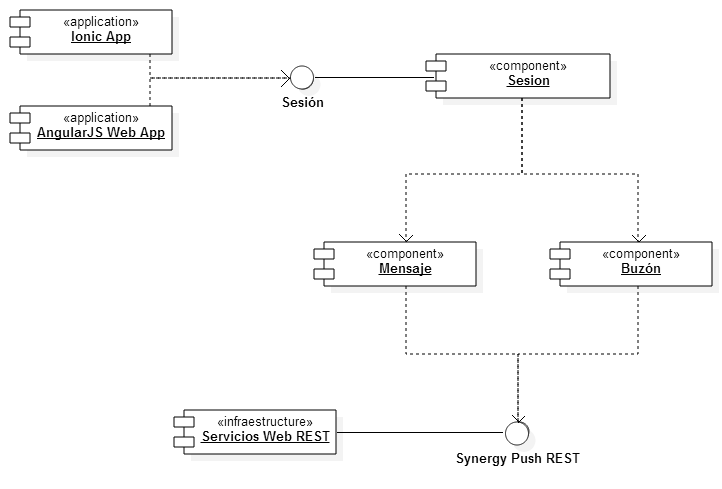
\includegraphics[scale=0.5,type=png,ext=.png,read=.png,angle=0,origin=c]{imagenes/Diagrama_de_Componentes}
  \caption{Diagrama de Componentes de Notificaciones+. Elaboración propia.}
  \label{fig:componentes}
\end{figure}


En este diagrama se puede observar el patrón de diseño MVC (Model-View-Controller) ya que cada capa representa un elemento de los anteriores, se aprecia como Ionic App y AngularJS Web App representan la capa de las vistas (View). Para el caso de la Sesión y cada uno de los siguientes dos componentes: Mensaje y Buzón, representan, en conjunto, el controlador (Controller). Y para finalizar, la capa de servicios de Notificaciones+ representa los datos o el modelo como tal (Model).


\subsubsection{Vista de Implantación}
La vista de implantación de la arquitectura de Notificaciones+ se ve reflejada en el Diagrama de Despliegue que se muestra en la Figura ~\ref{fig:despliegue}

\begin{figure}[H]
  \centering
  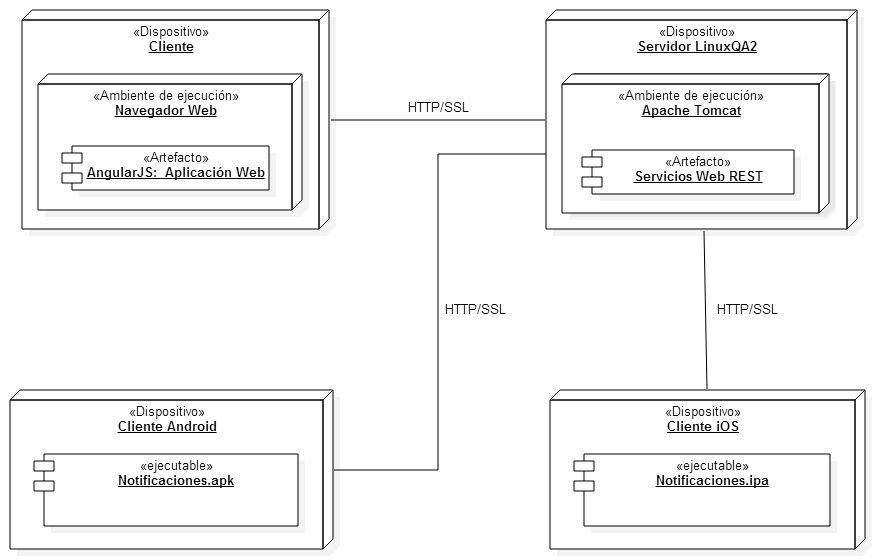
\includegraphics[scale=0.4,type=png,ext=.png,read=.png,angle=0,origin=c]{imagenes/Diagrama_de_Despliegue}
  \caption{Diagrama de Despliegue de Notificaciones+. Elaboración propia.}
  \label{fig:despliegue}
\end{figure}


Se puede ver como co-existen las aplicaciones móviles (para Android y iOS) junto con la aplicación web, e interactúan con los servicios web Rest cuando las aplicaciones se encuentran todas desplegadas.
Es importante aclarar que la comunicación se realiza a través de HTTP debido a que la plataforma Synergy Push todavía es un prototipo. Posteriormente cada una de estas se comunicará a través de HTTPS/SSL. La información que se comparte entre los nodos se encuentra en formato JSON.


\subsubsection{Vista de Procesos}
La Vista de Procesos no fue desarrollada, dado que la aplicación no resuelve aspectos de concurrencia de usuarios y de datos. Los mismos son resueltos por la arquitectura Synergy Push y el sistema bancario al que se instancie la aplicación.


\subsubsection{Vista de Datos}
La Vista de Datos no fue desarrollada dado que la aplicación como tal no cuenta con una base de datos propia. Ésta se alimenta de datos provistos por un core bancario debido al marco de trabajo de Synergy-GB. 


Es importante mencionar que cuando la aplicación sea instanciada para algún banco particular, se alimentará de los datos expuestos por dicho banco. Esos datos corresponden a los atributos de las clases del diagrama de clases mostrado en la Figura  ~\ref{fig:clases}.


\subsection{Planificación del desarrollo}
Se armó un plan inicial de desarrollo basado en los objetivos del proyecto descritos en la introducción del presente informe, lo que se planteaba en el plan de trabajo y los requerimientos que se levantaron junto con el cliente.
Este plan consta de cuatro iteraciones, de unas 4 semanas de duración cada una, aproximadamente. El mismo sufrió varios cambios a medida que se implementaban las funcionalidades para incluir actividades que no habían sido previstas, reestablecer prioridades en el desarrollo, y demás actividades que permitiesen gestionar los cambios en el proceso de construcción. En la Tabla ~\ref{table:iteraciones} se describen los objetivos de cada iteración.


\begin{table}
%\centering 
\begin{tabular}{| p{2.5cm} | p{13.5cm} |}
\hline 
\bfseries \footnotesize {Iteración} & \bfseries \footnotesize {Objetivos finales} \\ 
\hline 
\bfseries \footnotesize {Iteración 1} & 
\begin{itemize}[noitemsep,nolistsep]
  \item \footnotesize Diseño detallado e implementación del módulo de notificaciones y alertas e integración con Synergy Push:
  \begin{itemize}[noitemsep,nolistsep]
    \item \footnotesize Envío de notificaciones interactivas y recepción de respuestas
    \item \footnotesize Envío de información promocional con contenido Web
    \item \footnotesize Envío de recibos de transacciones realizadas en otros canales
  \end{itemize}
\end{itemize}
\\ \hline 
\bfseries \footnotesize {Iteración 2} & 
\begin{itemize}[noitemsep,nolistsep]
  \item \footnotesize Diseño detallado e implementación de la aplicación móvil y web de notificaciones y alertas:
  \begin{itemize}[noitemsep,nolistsep]
	   \item \footnotesize Gestión de notificaciones y respuestas
  \end{itemize}
  \item \footnotesize  Diseño detallado e implementación de la aplicación móvil en phonegap, para las funcionalidades de notificación y alertas
\end{itemize}
\\ \hline 
\bfseries \footnotesize{Iteración 3} & 
\begin{itemize}[noitemsep,nolistsep]
  \item \footnotesize Diseño detallado e implementación de la aplicación móvil en phonegap incluyendo todas sus funcionalidades. 	
\end{itemize}
\\ \hline 
\bfseries \footnotesize{Iteración 4} & 
\begin{itemize}[noitemsep,nolistsep]
  \item \footnotesize Prueba de la aplicación móvil en las distintas plataformas móviles, y desarrollo de ajustes para problemas específicos de plataformas.
  \item \footnotesize Finalización de los casos pendientes de las iteraciones anteriores.  
\end{itemize}
\\ \hline 
\end{tabular}
\footnotesize \caption{Iteraciones de desarrollo de Notificaciones+ y sus objetivos. Elaboración Propia.}
\label{table:iteraciones}
\end{table}


\section{Construcción} \label{sect:Construccion}
Esta fase se centró en el desarrollo de las funcionalidades y Casos de Uso previamente definidos, siguiendo la planificación especificada en la Tabla ~\ref{table:iteraciones}. La misma se llevó a cabo de acuerdo a los estándares de Synergy-GB promoviendo la modularidad, reutilización y gerencia de cambio (cambios de requisitos de \textit{software} no planificados).


Al finalizar cada iteración, los componentes desarrollados fueron probados para permitir la verificación de la correctitud de las funcionalidades implementadas. Al finalizar esta etapa, dichos componentes quedaron listos para pasar a las pruebas de sistemas y de aceptación, las cuales, sobre la base de la metodología que se está utilizando (Metodología de Proyectos de Synergy-GB), se hacen en la fase de transición.


\subsection{Iteración 1}
En esta iteración se realizaron las tareas de los Sprint 1, 2, 3 y 4 (pueden consultarse a detalle en el Apéndice C). Para cumplir los objetivos propuestos para esta etapa, en primer lugar, se realizó un estudio del API de la plataforma Synergy Push y de los requerimientos detallados del dueño del producto para realizar un diseño preliminar de la aplicación móvil, incluyendo las vistas. De la plataforma Synergy Push se dio a entender 2 distinciones esenciales del funcionamiento de la aplicación y de qué es lo que va a recibir y manejar:
\smallskip
\begin{itemize}[noitemsep,nolistsep]
  \item Notificaciones que alertan al usuario que posee un mensaje. Una notificación posee toda la información del mensaje excepto su contenido. El usuario puede recibir notoficaciones de dos maneras distintas:
  \begin{itemize}[noitemsep,nolistsep]
    \item Vía Push: exclusivo para dispositivos móviles. Son recibidos siempre y cuando el usuario haya hecho login, aún así el dispositivo esté en descanso y bloqueado.
    \item Vía HTTP: se reciben dentro de la aplicación, tanto móvil como web, a solicitud del usuario. Siempre se puede recibir la notificación de un mensaje mientras éste no haya sido abierto.
  \end{itemize}
  \item Mensajes: versión completa de la notificación, que posee un contenido de texto o dirección web. Una vez abierto se elimina de la plataforma Synergy Push y quedará contenido en el dispositivo móvil o en el navegador dónde el usuario lo haya abierto con la aplicación web.
\end{itemize}
\bigskip


En segundo lugar, una vez entregada una versión inicial de los diseños de vistas y funcionalidades, se procedió a empezar a implementar las vistas preliminares a la espera de las vistas oficiales del departamento de diseño. Una vez hechas las vistas preliminares se pasó a implementar las funcionalidades básicas de transición.


Al ser recibido el diseño de la aplicación del departamento de diseño de la empresa se pasó a adaptar las vistas ya hechas. Las vistas no eran convencionales y no se podían hacer con las utilidades que trae Ionic por defecto, así que se tuvo que hacer mucha investigación y experimentación para manipular el código CSS para lograr lo exigido.


Luego, se empezó la integración de lo ya programado a la plataforma Android y así empezar a implementar la recepción de las notificaciones Push, fundamentales para esta aplicación. Debido a la naturaleza experimental de esta funcionalidad, nueva en el framework Ionic, requirió gran cantidad de tiempo y pruebas, exclusivamente en Android; la creación de la versión móvil iOS se dejó para después de que la versión Android tuviera todas sus funcionalidades fundamentales implementadas, a petición del líder de movilidad de la empresa encargado de supervisar el proyecto.


Al finalizar esta iteración se hicieron pruebas manuales por parte del desarrollador usando directamente la plataforma Synergy Push para probar la recepción y el manejo de las notificaciones Push. Haciendo esto se descubrieron varios de los errores superados en la sección de Retos y Logros.


\subsection{Iteración 2}
En esta iteración se realizaron las tareas de los Sprint 5 y 6 (pueden consultarse a detalle en el Apéndice C), que incluyen las funcionalidades: login, apertura y recepción de mensajes, eliminar mensajes, registro y modificar perfil. Se tuvo que hacer también las vistas de registro y modificar perfil ya que no habían sido tomadas en consideración por el departamento de diseño ni el dueño del producto, para esto fue necesario que el desarrollador y el líder de departamento de diseño las hicieran en conjunto.


En esta iteración estaba planificado la implementación del grueso de las funcionalidades de la aplicación móvil multiplataforma y el comienzo de la aplicación web, con la intención de empezar la aplicación web desde cero, pero después de hecha la estructura principal se tomó la decisión de usar una plantilla web propiedad de la empresa, que no estaba lista todavía, así que todo lo que era desarrollo web fue postergado para la última iteración.


La aplicación está diseñada para trabajar en conjunto con la plataforma Synergy Push y con algún sistema del cliente que compre la aplicación, y como dicho sistema no existe todavía hay algunas cosas que tuvieron que resolverse:
\smallskip
\begin{itemize}[noitemsep,nolistsep]
  \item La aplicación debe iniciar sesión con la página del cliente (un banco u otro) así que se creo un mini servidor que aceptara inicio de sesión con el específico único de implementar esta funcionalidad.
  \item La aplicación debe registarse con Synergy Push y el sistema del cliente al mismo tiempo así que se hizo uso nuevamente del mini servidor provisional para que aceptara registro de la aplicación tanto web como móvil.
  \item Los mensajes deberían ser enviados por el sistema del cliente a la plataforma Synergy Push y es ésta la que lo gestiona y envía a la aplicación de los usuarios particulares. Para implementar y hacer pruebas de esto simplemente se hizo uso del modo desarrollador de Synergy Push y se enviaron los mensajes manualmente.
  \item Las respuestas de los mensajes interactivos son recibidas por el mismo sistema del cliente que envió dichos mensajes en primer lugar, para eso nuevamente se hizo uso del mini servidor provisional que recibiera las respuestas.
\end{itemize}
\bigskip


Luego se pasó a agregar guardado de mensajes persistente en la aplicación móvil, de manera que los mensajes abiertos no se perdieran hasta que el usuario los borrara.


Luego se exportó todo lo hecho tanto a la plataforma Android como a la plataforma iOS, descubriendo el error de Synergy Push para enviar notificaciones Push para iOS. La habilidad de recibir notificaciones Push por parte de la aplicación móvil fue comprobada por el desarrollador por medio de otros programas auxiliares. Todas las demás funcionalidades implementadas funcionan en ambas plataformas.


Al finalizar la iteración, se realizaron pruebas unitarias para todas las funcionalidades implementadas. Al igual que en la iteración anterior, estas pruebas fueron llevadas a cabo de forma manual utilizando la plaraforma Synergy Push y el mini servidor provisional.


\subsection{Iteración 3}
En esta iteración se realizaron las tareas de los Sprint 7 y 8 (pueden consultarse a detalle en el Apéndice C) que incluyen las funcionalidades: \textit{pull refresh}, autenticación, compartir mensajes y botones de respuesta, además del arreglo de un bug de la recepción Push para Android detectado por el desarrollador. Esta iteración consiste básicamente en terminar los últimos detalles y resolver los errores de la aplicación móvil.


Primero se implementó la funcionalidad \textit{pull refresh}, que simplemente consiste en darle poder al usuario para hacer que la aplicación buscara notificaciones nuevas desde el buzón vía HTTP sin tener que esperar que llegara la notificación vía Push. Se tuvo que hacer uso de un algoritmo muy eficiente para mezclar la lista de notificaciones entrante con la que ya estaba almacenada en el teléfono para ahorrar recursos computacionales del dispositivo. Este algoritmo consiste en una mezcla de listas de JavaScript usando la función "map()".

Luego se hizo la funcionalidad autenticar, que simplemente consistió en una mejora del login ya implementado. Se hizo que la aplicación mandara una solicitud en particular al mini servidor y que este devolviera a su vez una respuesta particular que le permitiera a la aplicación avanzar a la siguiente vista.


Para la funcionalidad de compartir solo se hizo uso del plugin de Cordova diseñado para eso, que funciona adecuadamente para ambas plataformas móviles y comparte los mensajes de Notificaciones+ a través de cualquier aplicación de mensajería o de red social que el usuario tenga instalada en su dispositivo. 


Los botones de respuesta se implementaron haciendo uso del mini servidor provisional para que recibiera dichas respuestas. Se tuvo una reunión con el dueño del producto y este indicó que los mensajes se podían responder solamente una vez y así fue implementado.


La última tarea del Sprint consistía en resolver un error de recepción Push en la versión Android de Notificaciones+, dónde las notificaciones Push no son recibidas por la aplicación si esta estaba en segundo plano. Se hizo investigación y varias pruebas hasta localizar el error en el código fuente del plugin de recepción Push. Para resolver esto se tuvo que modificar dicho código fuente para adaptarlo a las necesidades de la aplicación. Se desconoce si este error se presenta también para iOS ya que como se ha mencionado antes, la plataforma Synergy Push no es capaz de mandar notificaciones Push a iOS todavía.


\subsection{Iteración 4}
En esta iteración se realizaron las tareas de los Sprint 9, 10 y 11 (pueden consultarse a detalle en el Apéndice C) que abarca todo el desarrollo de la aplicación Notificaciones+ Web. Una vez obtenido acceso a la plantilla web de la empresa, se pasó a adaptar las partes útiles las necesidades de la aplicación tanto visual como en funcionalidad. Debido a que no era necesario hacer una vista desde cero sino adaptar una, los aspectos visuales fueron sugeridos directamente por el líder del departamento de diseño sin necesidad de realizar un diseño completo.


Primero se adaptó una vista de manejador de correo electrónico perteneciente a la plantilla para hacer de vista buzón de Notificaciones+. Luego se pasó a hacer las funcionalidades. Después de toda la experiencia adquirida en el desarrollo de la aplicación en Ionic, el desarrollo web fue relativamente sencillo. Una vez completadas todas las funcionalidades de la vista buzón, incluyendo filtro por tipo de mensajes y por texto introducido por el usuario, se pasó a desarrollar las siguientes vistas.


Las vistas y funcionalidades de login, registro y modificar perfil se adaptaron igualmente de las páginas prediseñadas de la plantilla. La pantalla de modificar perfil fue una adaptación de la de registro ya que no existía un equivalente en la plantilla. Sus funcionamientos fueron análogos a la versión móvil de Ionic, haciendo uso de las mismas técnicas de programación y del mini servidor provisional.


El último requisito que se atacó fue la vista de detalles de mensajes, y sus funcionalidades inherentes como compartir, eliminar y responder mensajes. La respuesta de mensajes es análoga a la de la aplicación móvil. La funcionalidad de eliminar mensajes no lo fue tanto ya que en la aplicación web se puede enviar los mensajes a una papelera desde el buzón antes de ser borrados y luego en la papelera se pueden eliminar varios o todos los mensajes al mismo tiempo seleccionándolos antes. Desde la vista de detalles de mensaje también se pueden borrar los mensajes pero solo definitivamente sin pasar por la papelera primero. La funcionalidad compartir requirío aplicar links directos a las redes sociales correspondientes excepto para Facebook, cuyas políticas de desarrollo obligan a registrar la aplicación Notificaciones+ para poder compartir algo.


Finalmente se hicieron pruebas manuales para verificar el correcto desempeño de todas las funcionalidades implementadas. 


\subsection{Descripción general del producto}
Al finalizar la fase de construcción, se cuenta con un prototipo funcional estable de Notificaciones+ tanto web como móvil, validado por el cliente. La aplicación permite: iniciar y cerrar sesión; recibir mensajes vía push o Internet, guardar los mensajes, compartir y eliminar mensajes.

Al abrir las aplicaciones, se muestra la pantalla de inicio de sesión, en la cual deben escribirse los datos del usuario para poder iniciar su sesión y entrar a su buzón. En la Figura ~\ref{fig:login} se muestra las capturas de pantalla de dicha vista (tanto para móvil como para web).

%%En la Figura ~\ref{fig:login} se muestra la pantalla de la página de inicio de sesión del sistema.
\begin{figure}[htp]
  \centering
  %%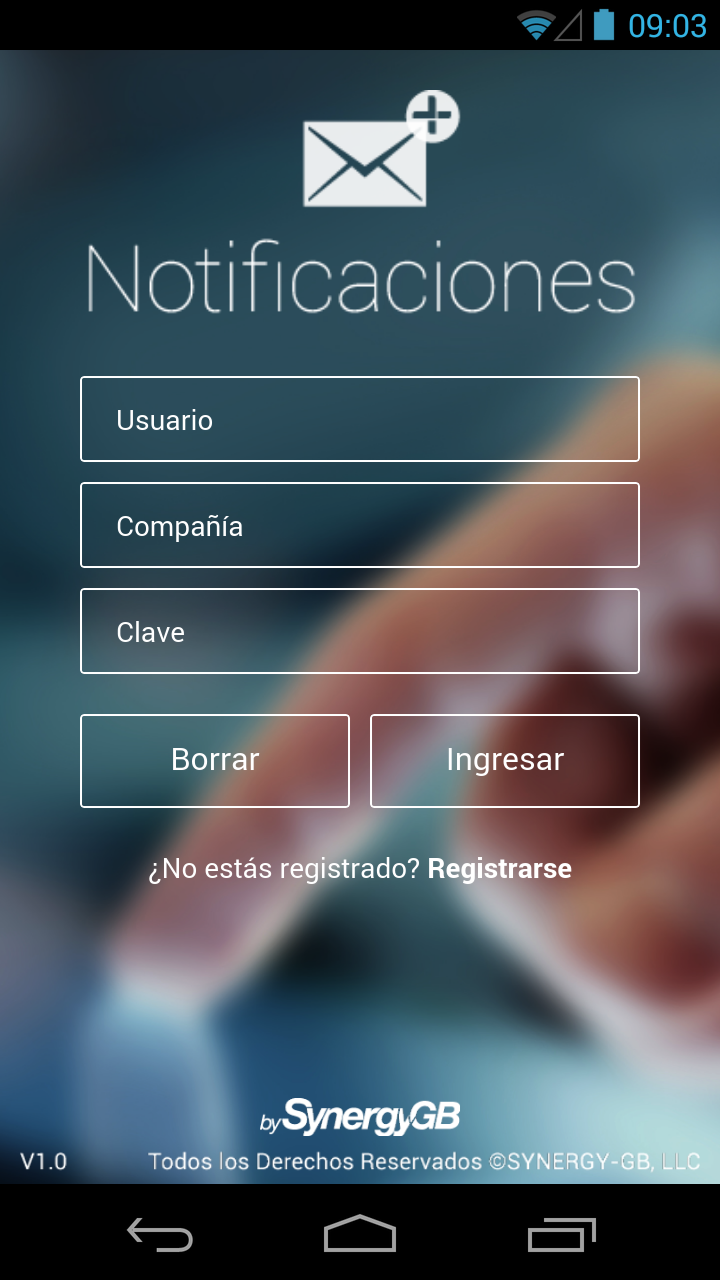
\includegraphics[width=3cm,type=png,ext=.png,read=.png,angle=0,origin=c]{imagenes/pantalla1}
  \subfloat[Versión Web]{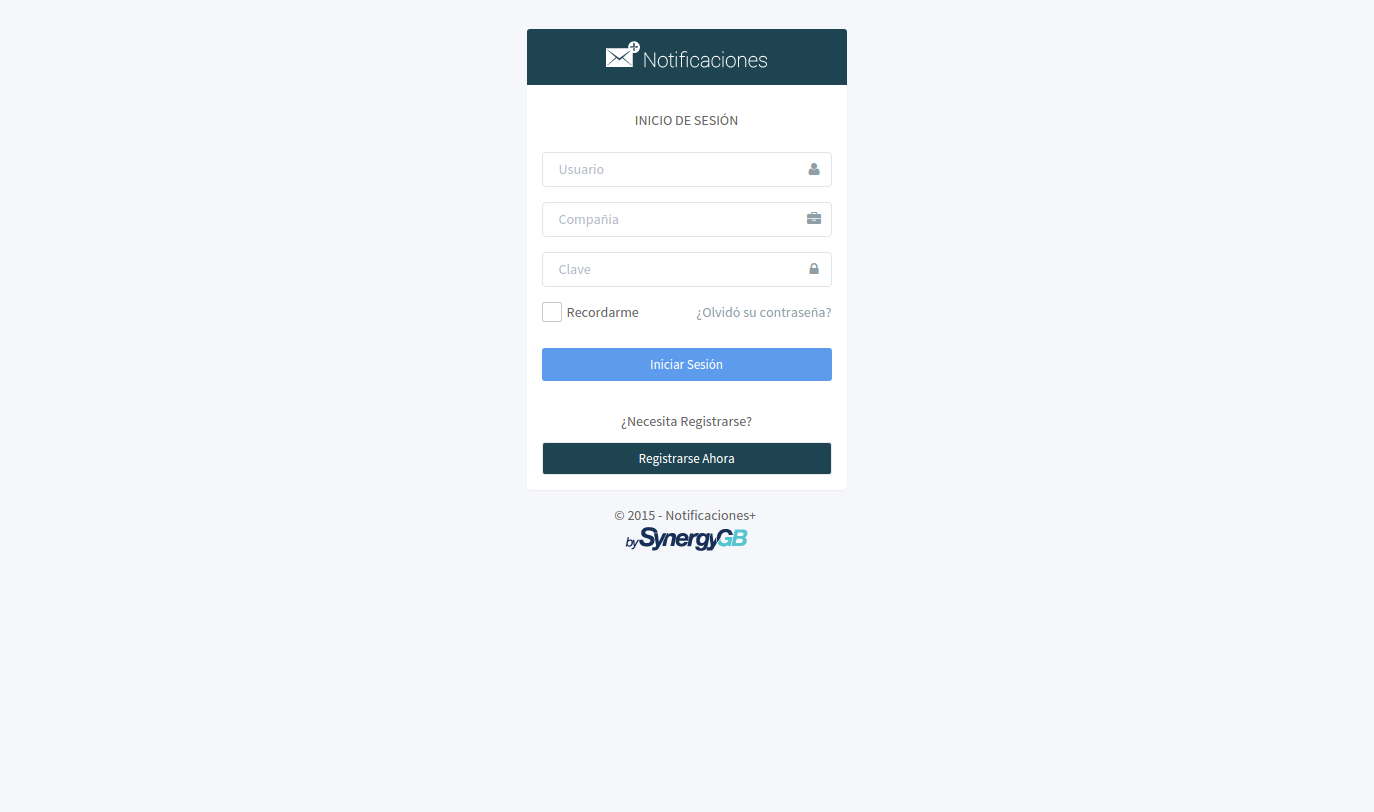
\includegraphics[width=11cm]{imagenes/Login_Web2}}
  \quad
  \subfloat[Versión Móvil]{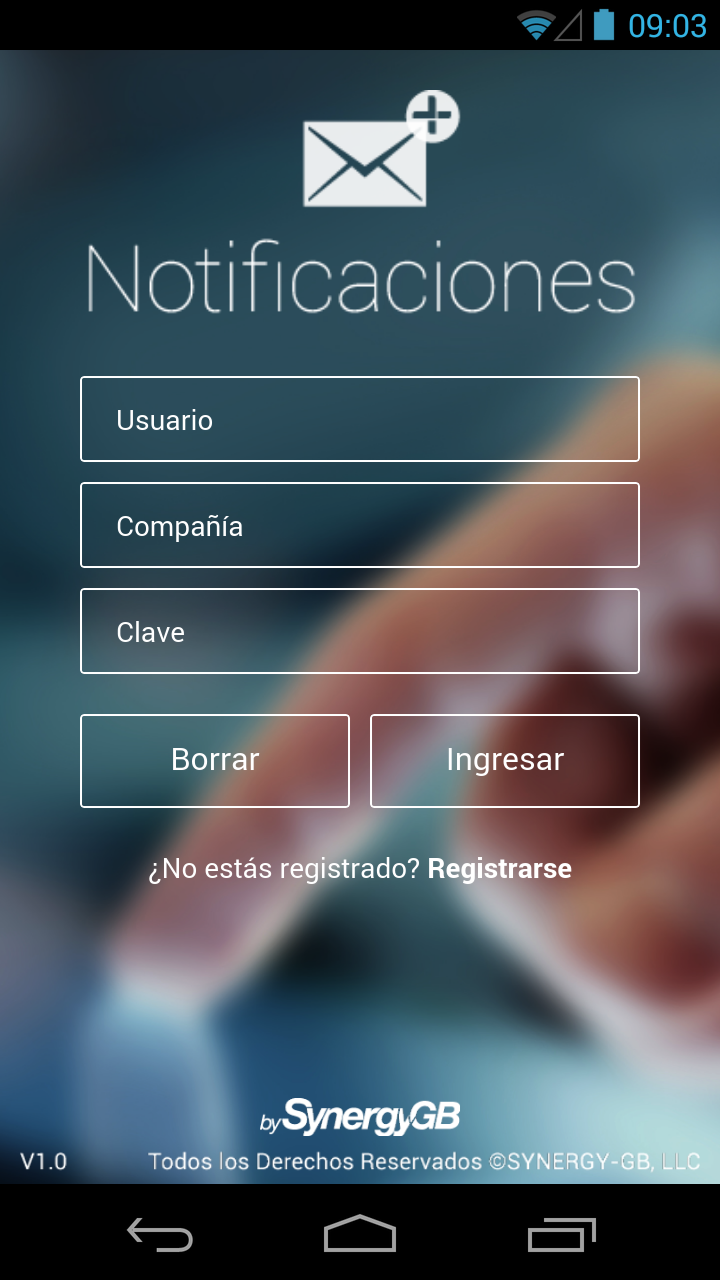
\includegraphics[width=3.5cm]{imagenes/pantalla1}}
  \caption{Pantallas de Inicio de Sesión de Notificaciones. Elaboración propia.}\label{fig:login}
\end{figure} 

Si el usuario no estrá registrado, se le da la opción al usuario de registrarse a la plataforma en la pantalla login. En la Figura ~\ref{fig:registro} se muestra la captura de pantalla de esta página.
\begin{figure}[htp]
  \centering
  %%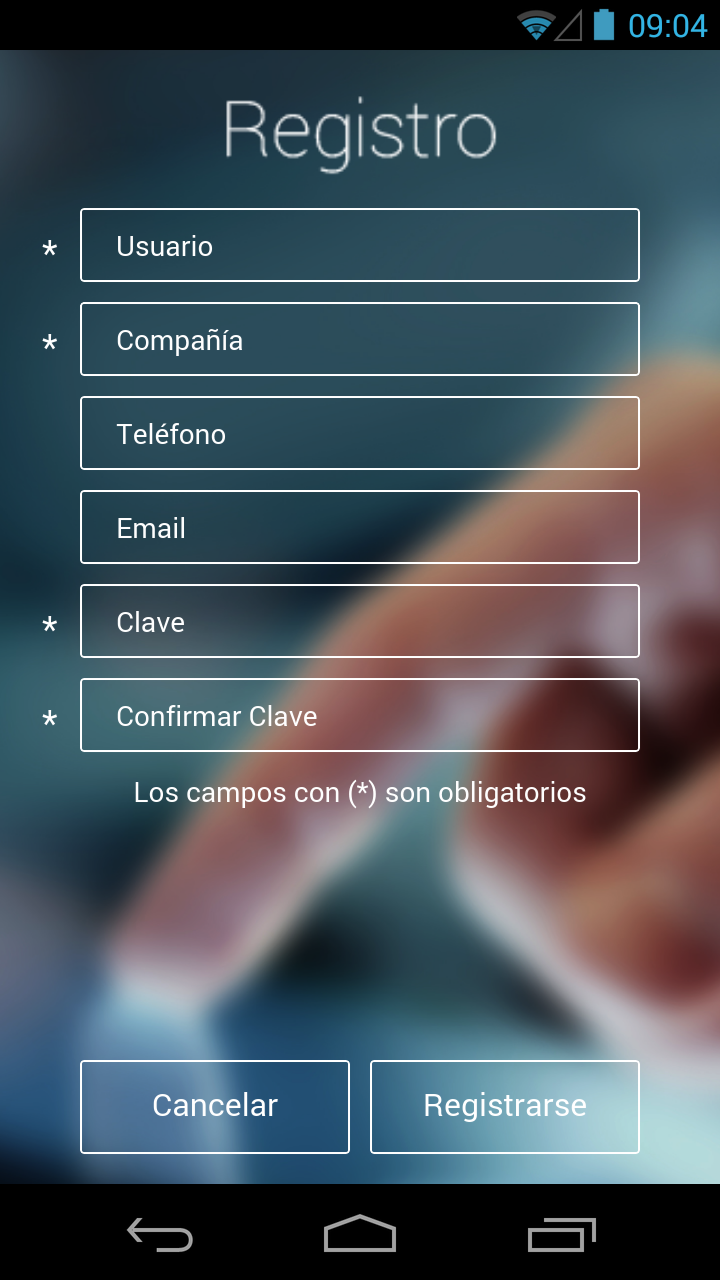
\includegraphics[width=3cm,type=png,ext=.png,read=.png,angle=0,origin=c]{imagenes/pantalla2}
  \subfloat[Versión Web]{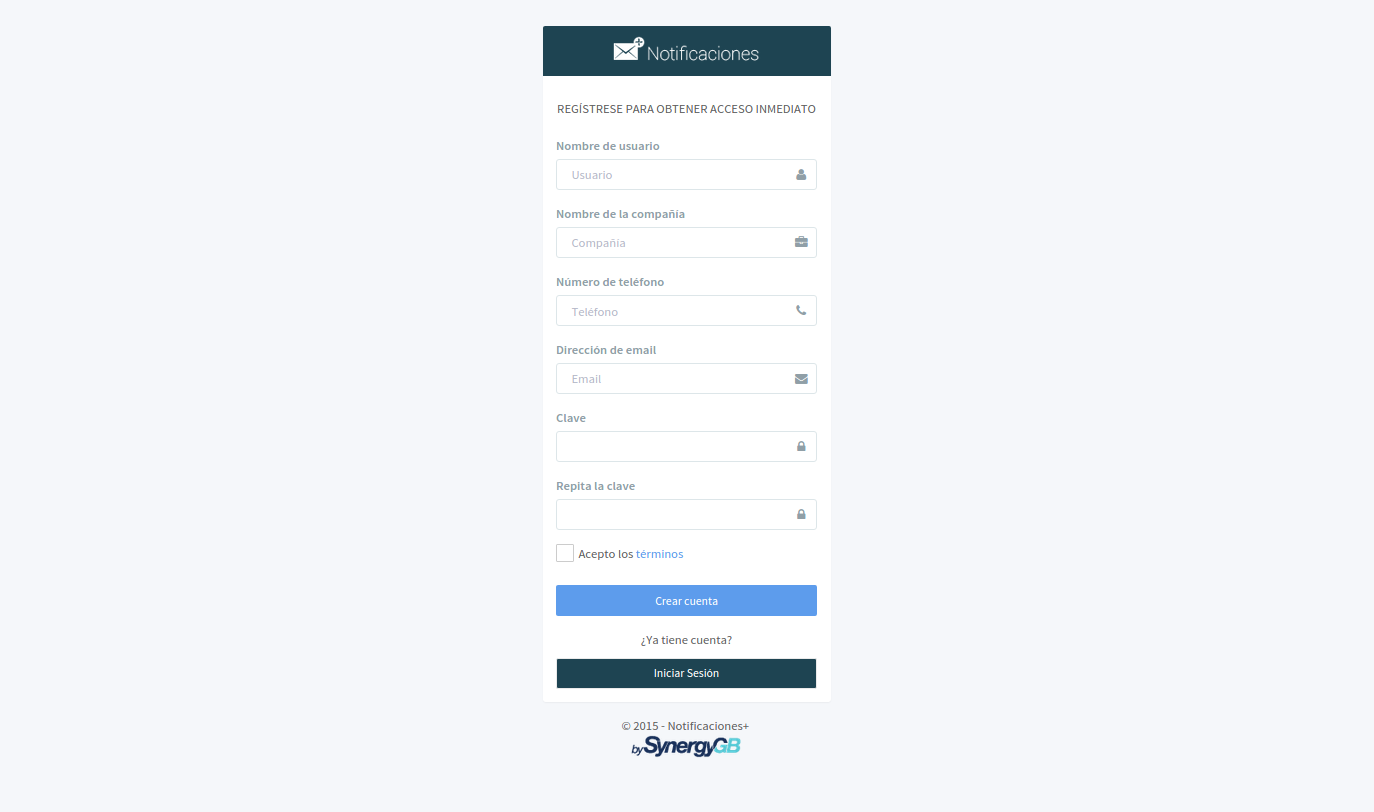
\includegraphics[width=11cm]{imagenes/Registro_Web2}}
  \quad
  \subfloat[Versión Móvil]{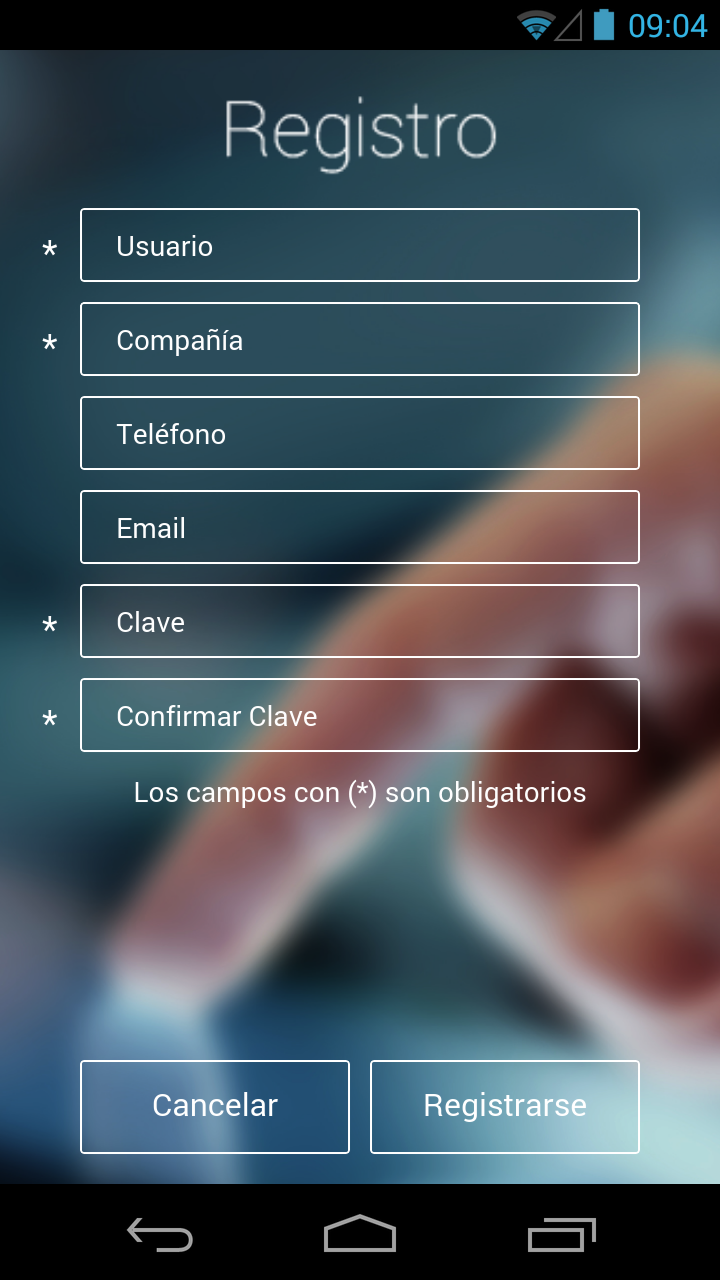
\includegraphics[width=3.5cm]{imagenes/pantalla2}}
  \caption{Pantalla de Registro. Elaboración propia.}\label{fig:registro}
\end{figure} 

Una vez iniciada la sesión del usuario se visualiza el menú principal, donde el usuario puede acceder directamente al buzón con o sin un filtro de mensajes seleccionado. Además, se le ofrece la opción de modificar su perfil. En la Figura ~\ref{fig:MenuPrincipal} se muestra la captura de pantalla de esta página.
\begin{figure}[htp]
  \centering
  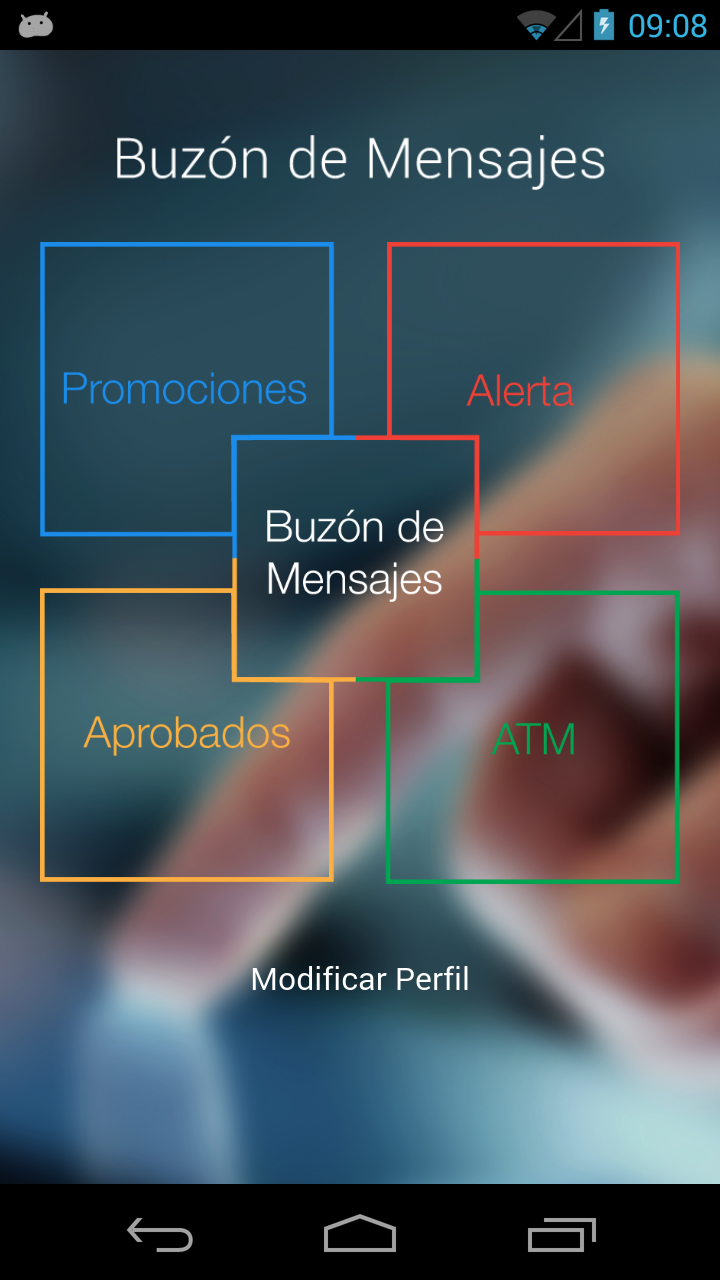
\includegraphics[width=3cm,type=png,ext=.png,read=.png,angle=0,origin=c]{imagenes/pantalla3}
  \caption{Pantalla de Menú Principal. Elaboración propia.}
  \label{fig:MenuPrincipal}
\end{figure} 

Si el usuario selecciona la opción de modificar su perfil se le muestra dicha pantalla, con el campo nombre en gris indicando que es lo único que no puede modificar. En la Figura ~\ref{fig:ModificarPerfil} se muestra la captura de pantalla de esta página, se puede acceder desde el Menú Principal en la aplicación móvil o desde el Buzón en la versión web.
\begin{figure}[htp]
  \centering
  %%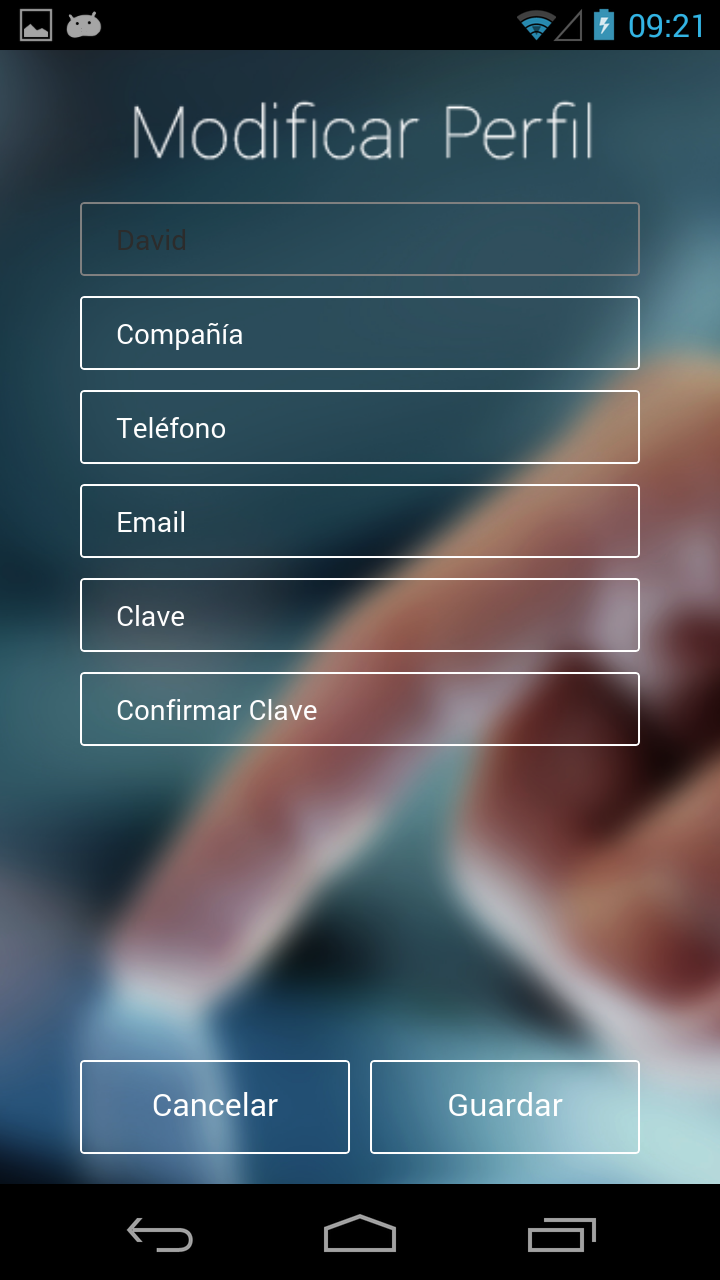
\includegraphics[width=3cm,type=png,ext=.png,read=.png,angle=0,origin=c]{imagenes/pantalla4}
  \subfloat[Versión Web]{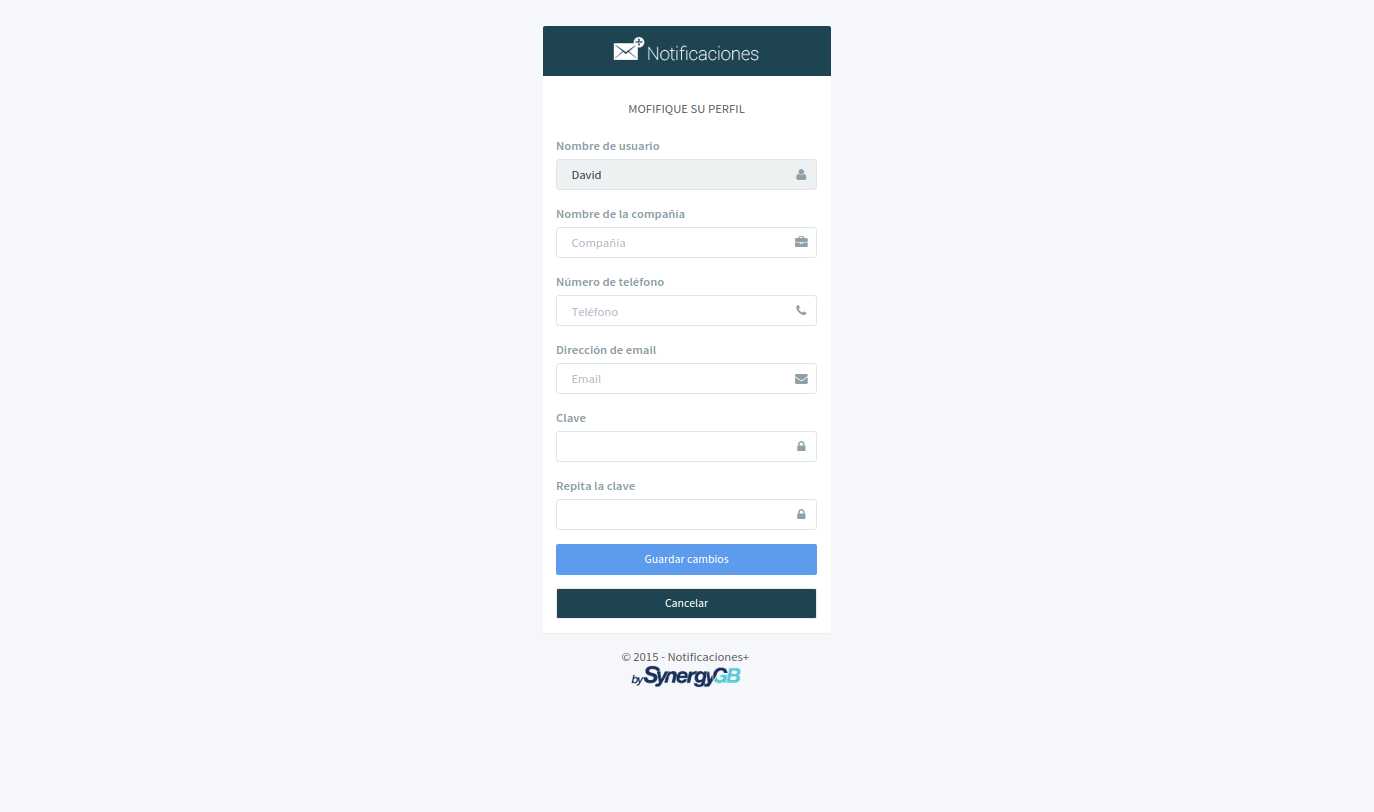
\includegraphics[width=11cm]{imagenes/Modificar_Perfil_Web2}}
  \quad
  \subfloat[Versión Móvil]{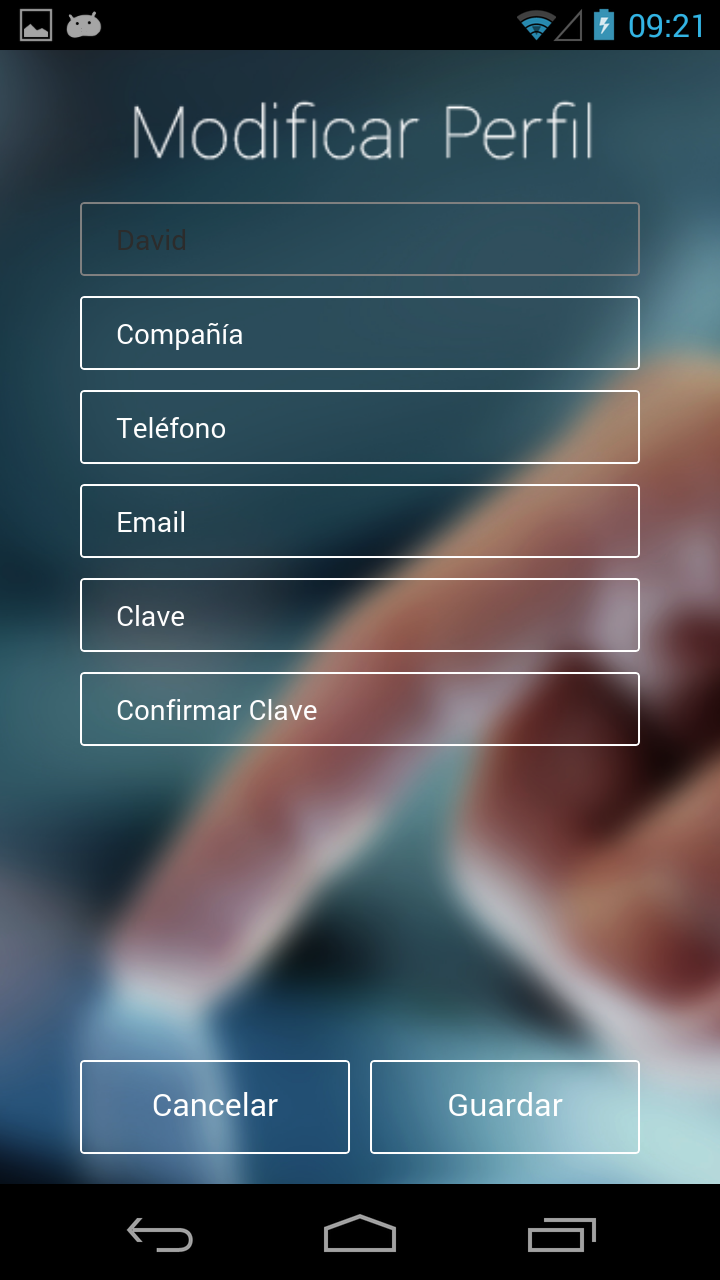
\includegraphics[width=3.5cm]{imagenes/pantalla4}}
  \caption{Pantalla Modificar Perfil. Elaboración propia.}
  \label{fig:ModificarPerfil}
\end{figure} 	

En la pantalla buzón, se muestran todos los mensajes recibidos, los cuales pueden ser filtrados por tipo al presionar uno de los botones mostrados, o por el texto que contienen en el cuadro de búsqueda. En la Figura ~\ref{fig:pantallaMulti} se puede observar la pantalla de la versión móvil sin alterar y bajo la acción de los botones. En la Figura ~\ref{fig:pantallaMultiWeb} se puede observar la pantalla de la versión web sin alterar y bajo la acción de los botones. Cabe acotar que para que aparezca el cuadro de búsqueda en la versión web hay que solicitarlo mediante el botón indicado.
\begin{figure}[htp]
\centering
  \subfloat[Buzón de mensajes]{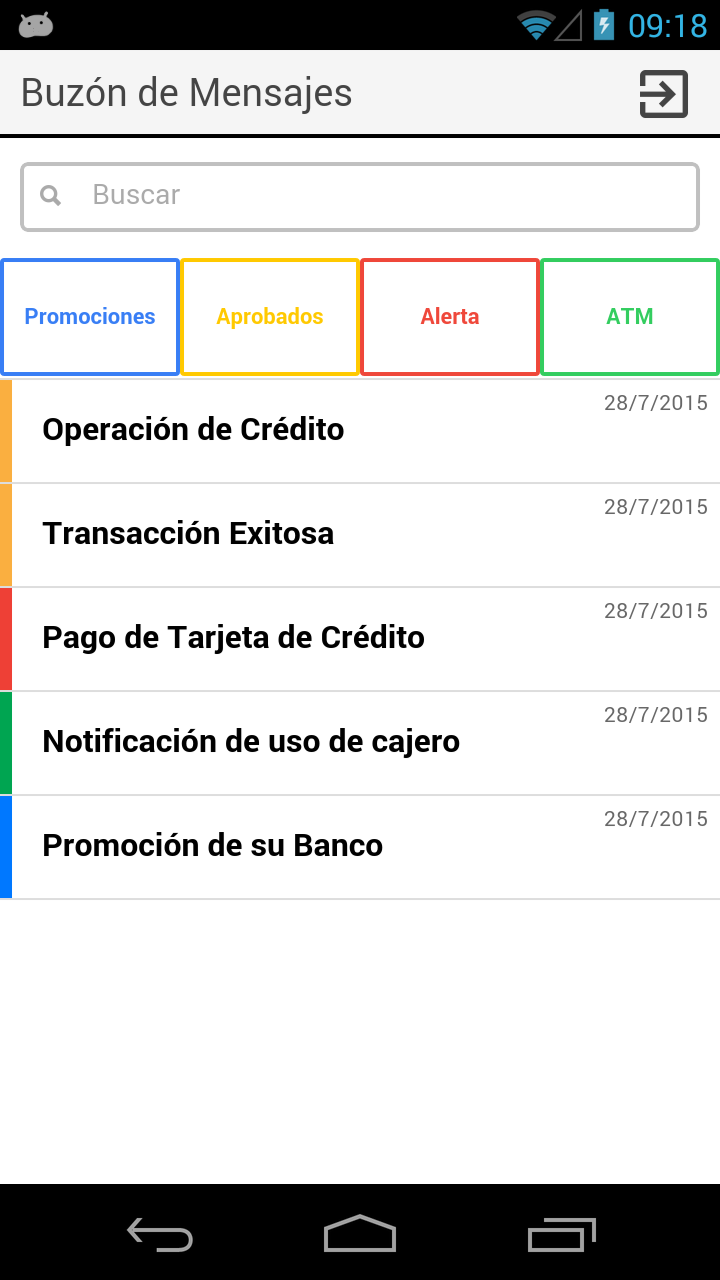
\includegraphics[width=3.5cm]{imagenes/pantalla5}}
  \quad
  \subfloat[Filtro Aprobados]{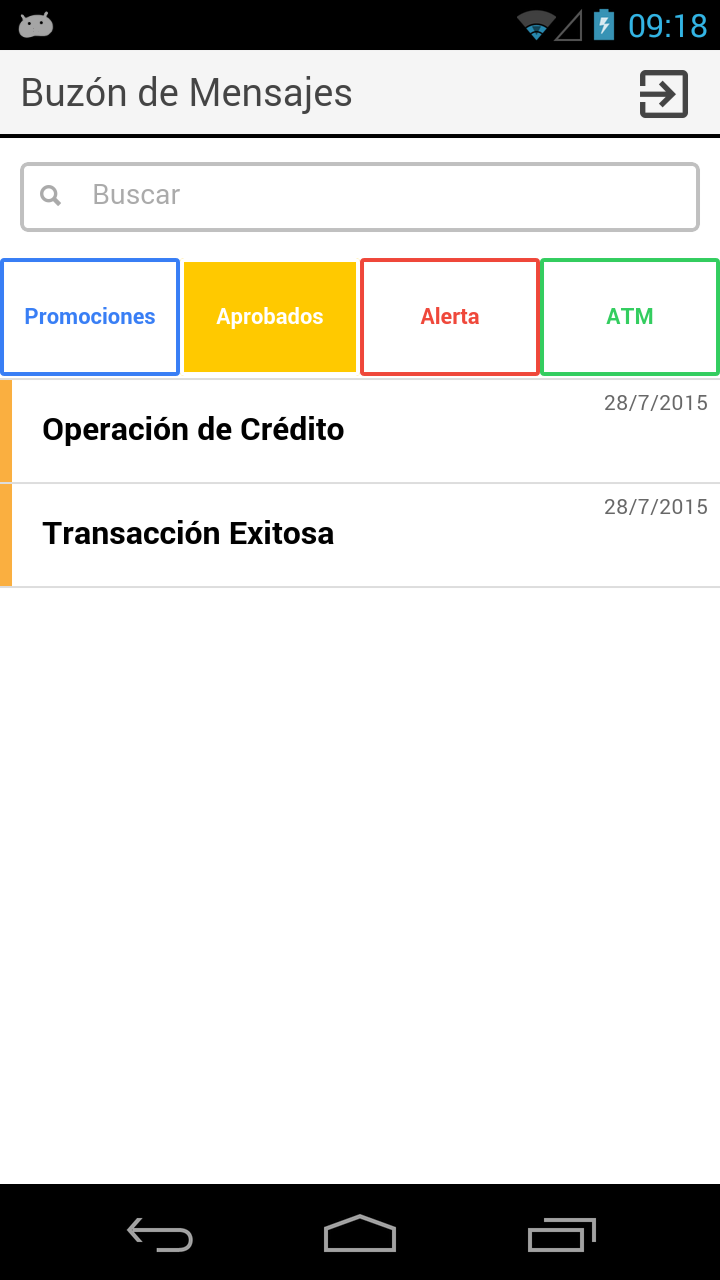
\includegraphics[width=3.5cm]{imagenes/pantalla6}}
  \quad
  \subfloat[Filtro Promociones]{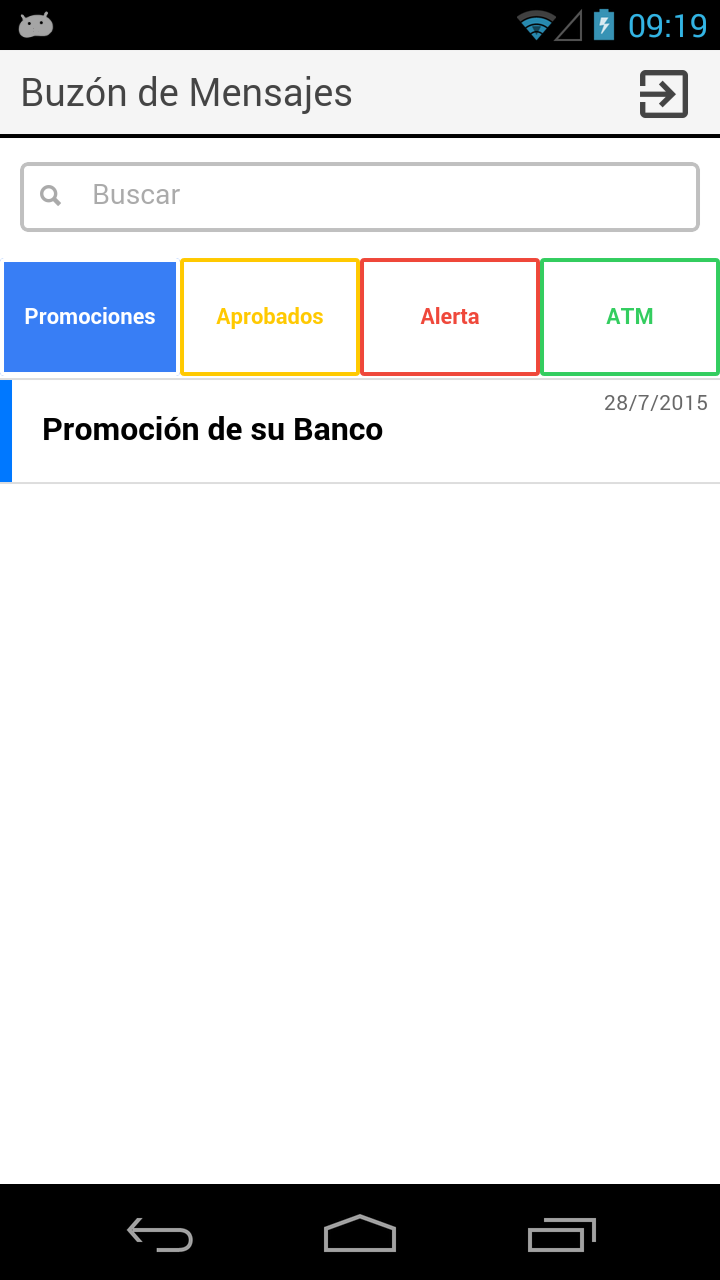
\includegraphics[width=3.5cm]{imagenes/pantalla7}}
  \quad
  \subfloat[Filtro Alerta]{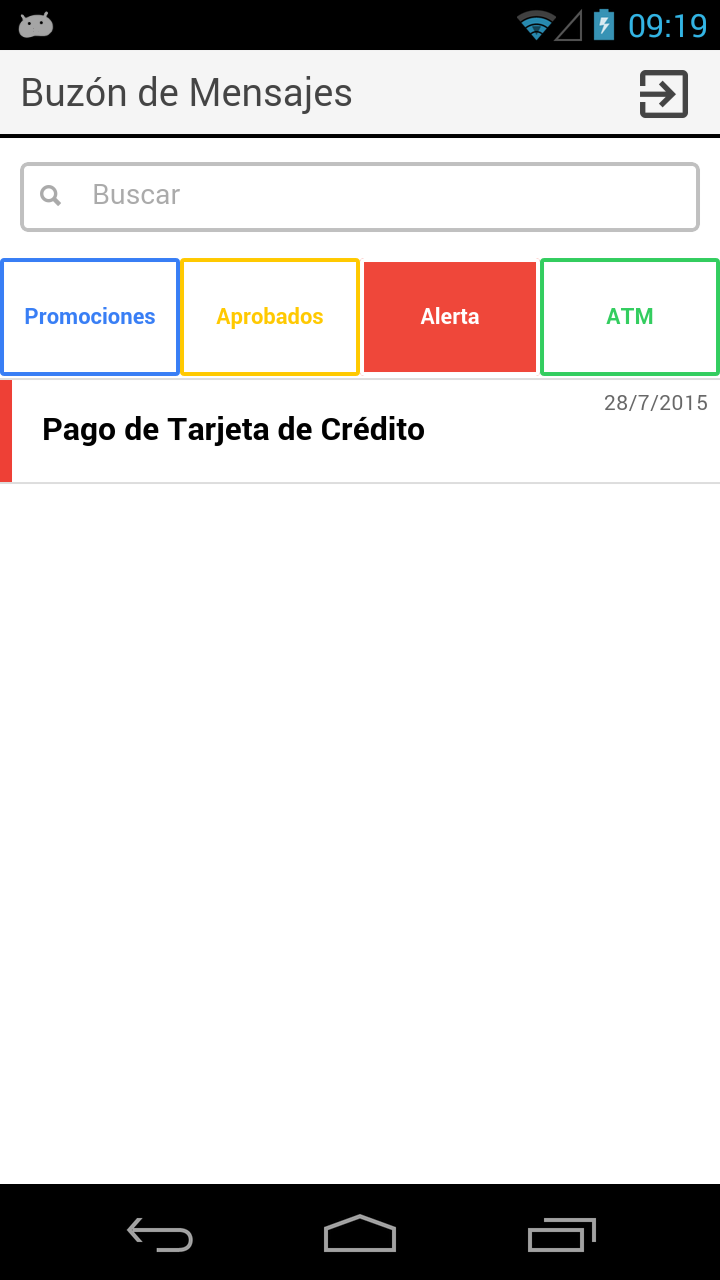
\includegraphics[width=3.5cm]{imagenes/pantalla8}}
  \quad
  \subfloat[Filtro ATM]{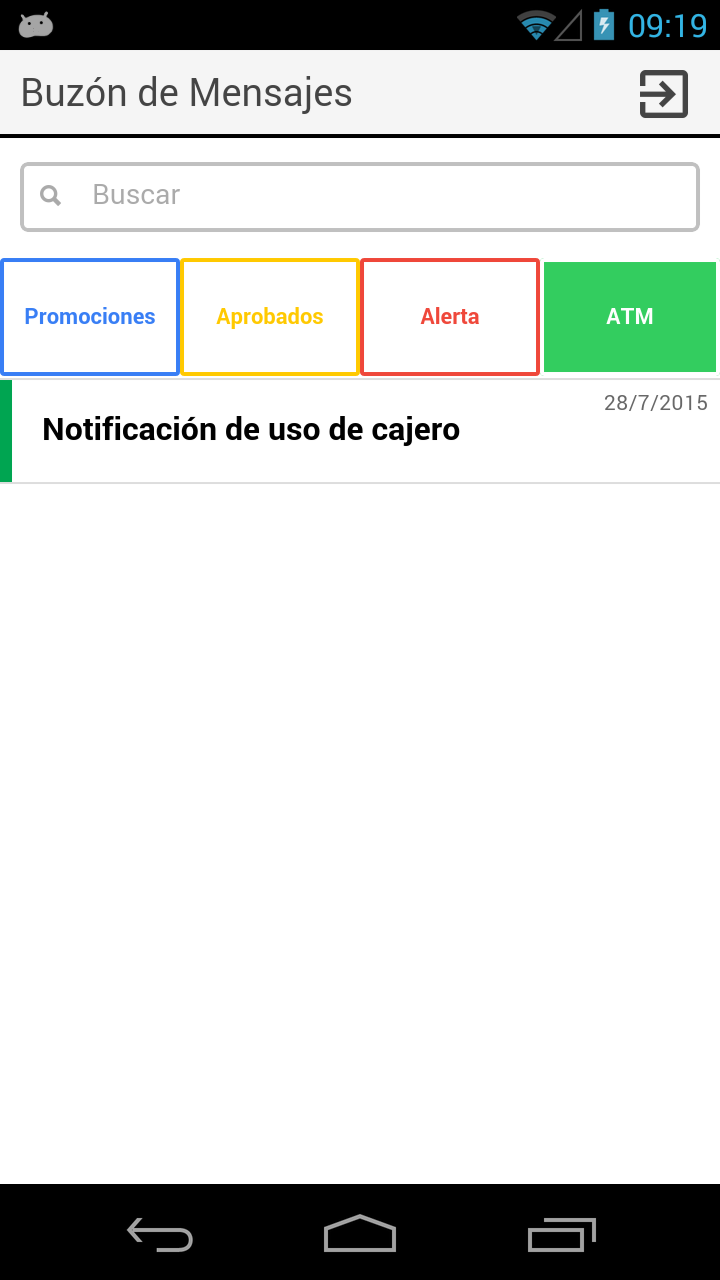
\includegraphics[width=3.5cm]{imagenes/pantalla9}} 
  \quad
  \subfloat[Mensaje leído]{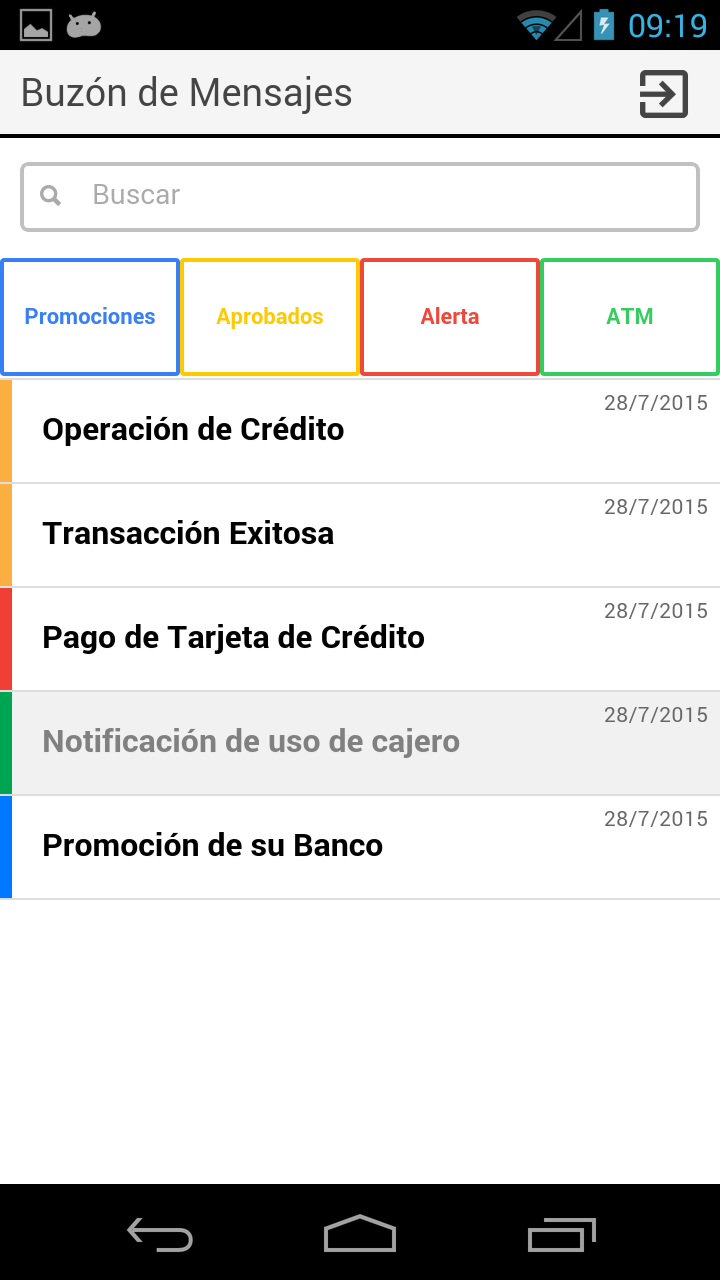
\includegraphics[width=3.5cm]{imagenes/pantalla10}}
\caption{Pantalla de Buzón con botones de filtrado versión Móvil. Elaboración propia.}\label{fig:pantallaMulti}
\end{figure}

\begin{figure}[htp]
\centering
  \subfloat[Buzón de mensajes]{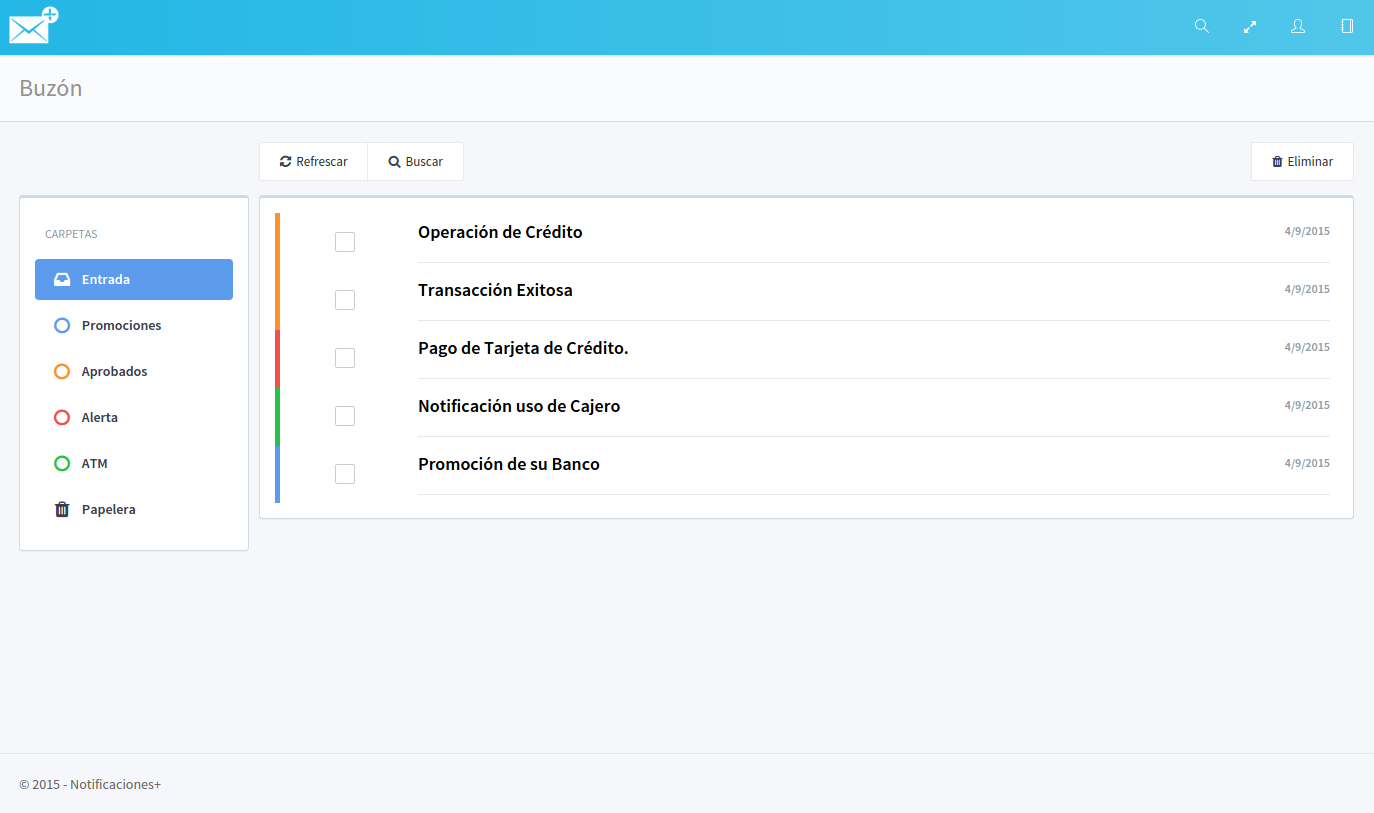
\includegraphics[width=11cm]{imagenes/Buzon_Web}}
  \quad
  % \subfloat[Filtro Aprobados]{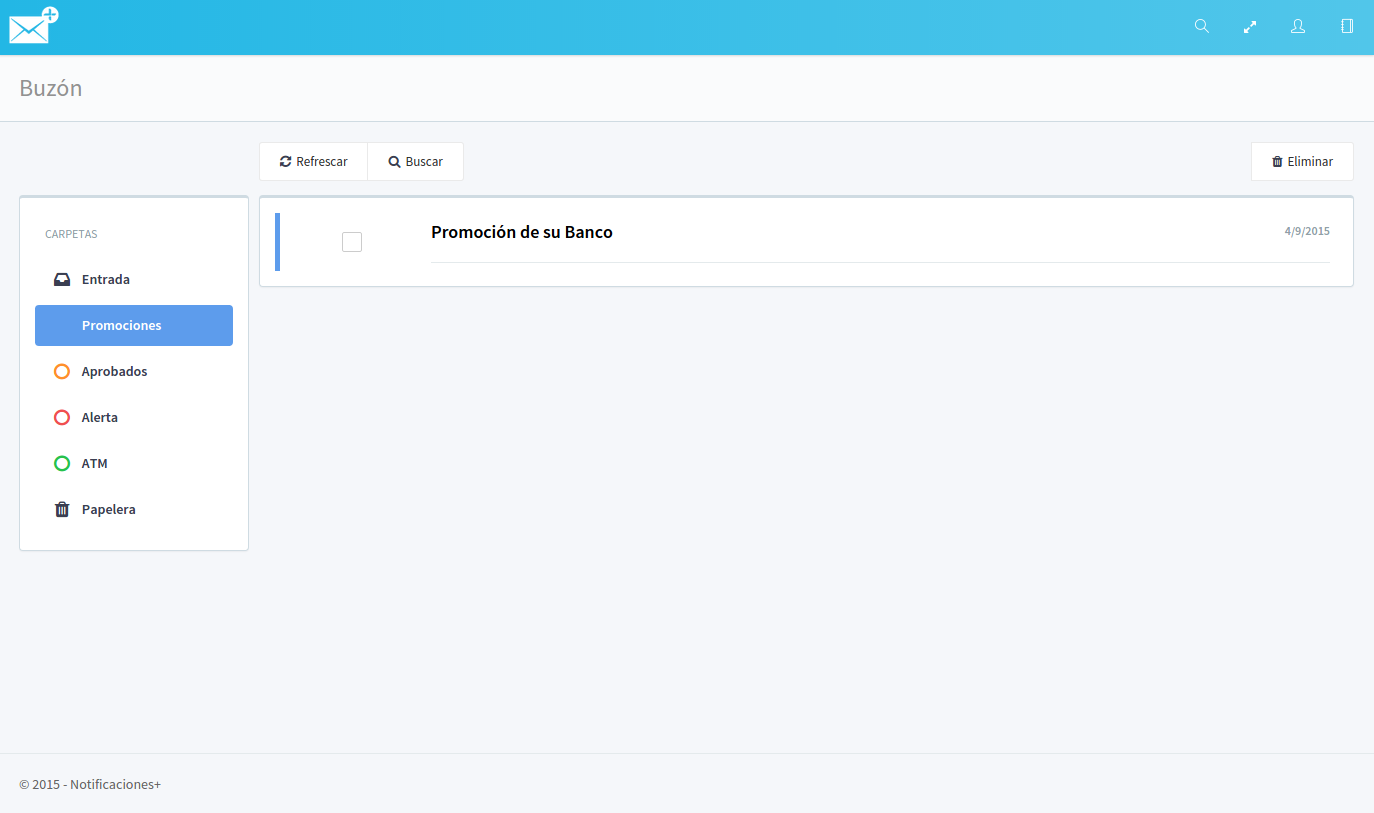
\includegraphics[width=11cm]{imagenes/Filtro1}}
  % \quad
  % \subfloat[Filtro Promociones]{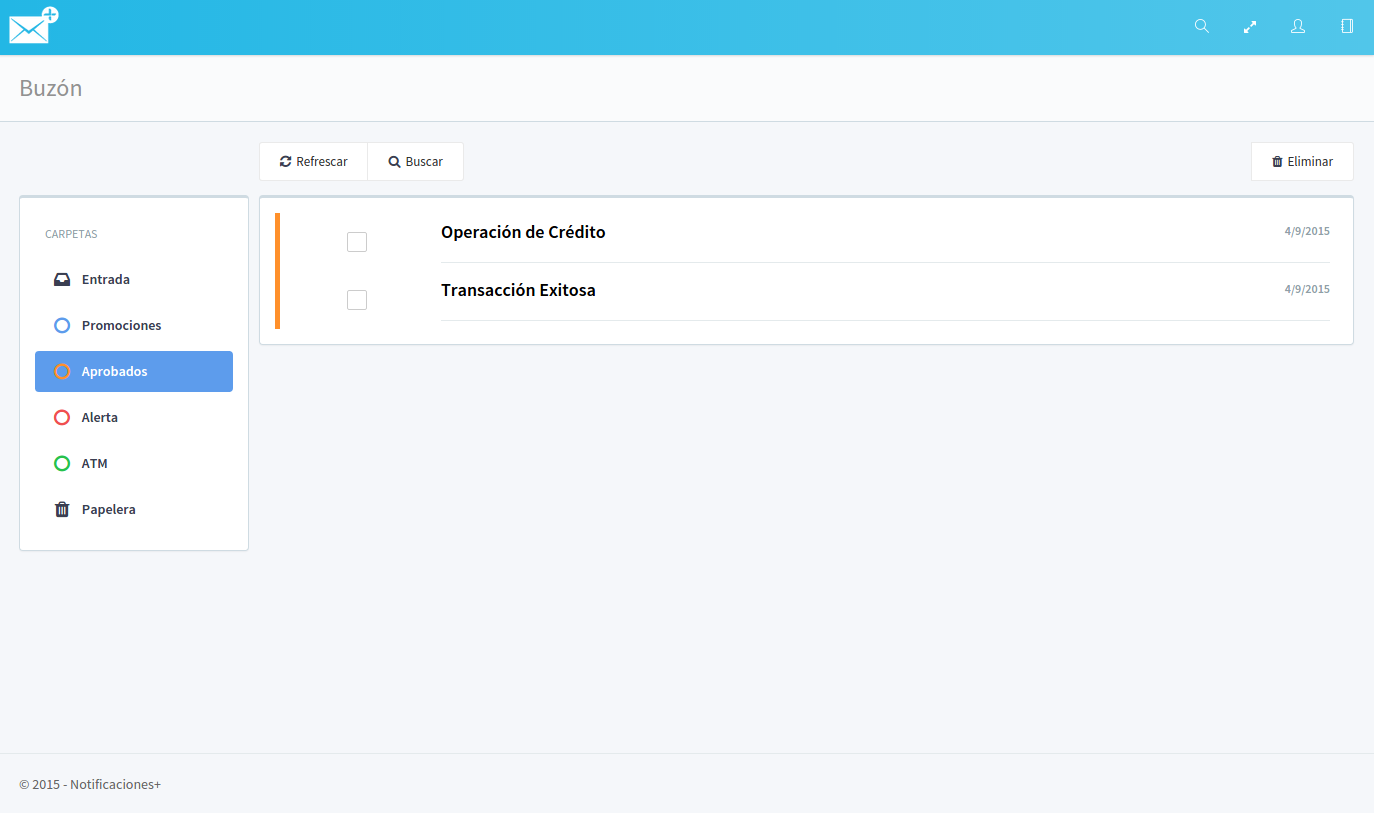
\includegraphics[width=11cm]{imagenes/Filtro2}}
  % \quad
  % \subfloat[Filtro Alerta]{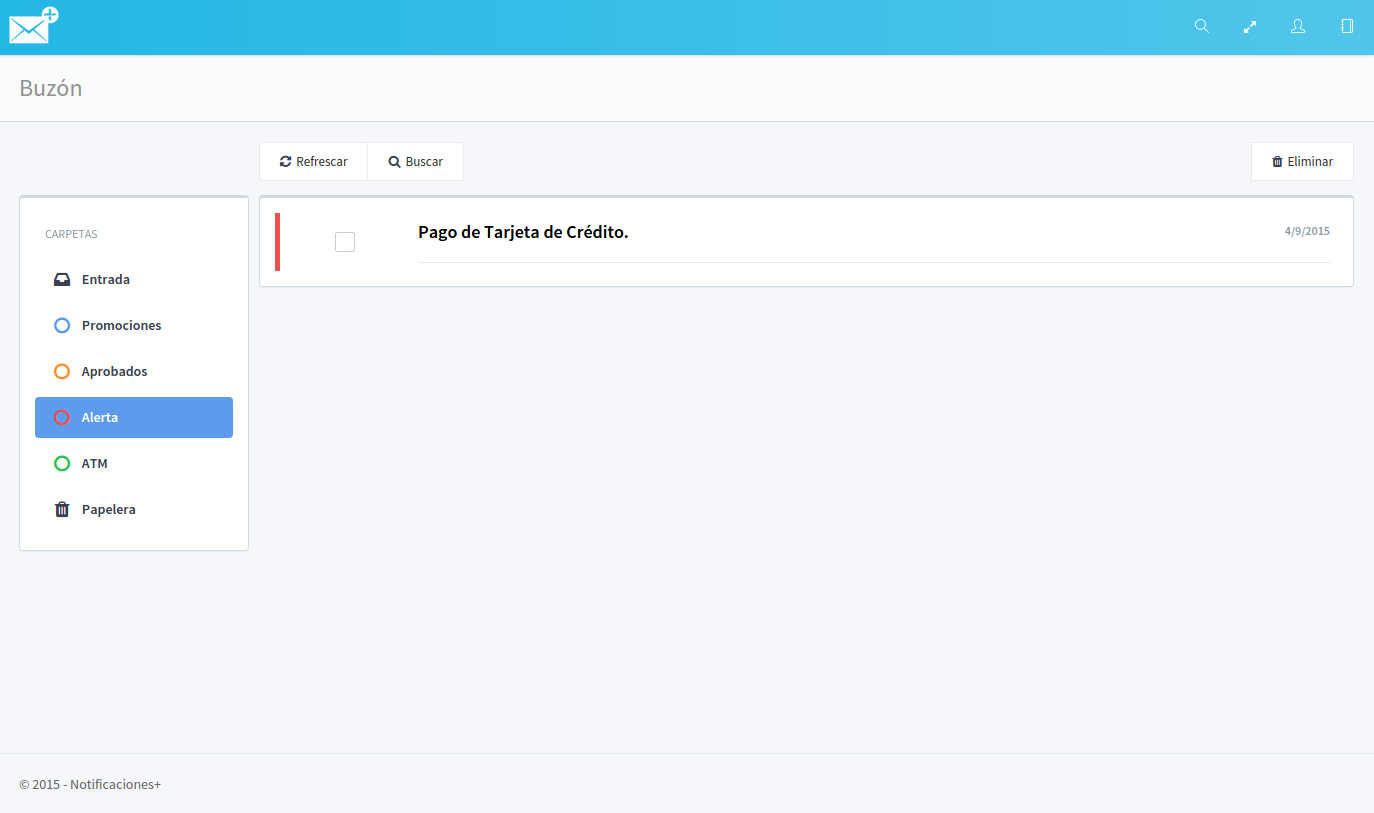
\includegraphics[width=11cm]{imagenes/Filtro3}}
  % \quad
  % \subfloat[Filtro ATM]{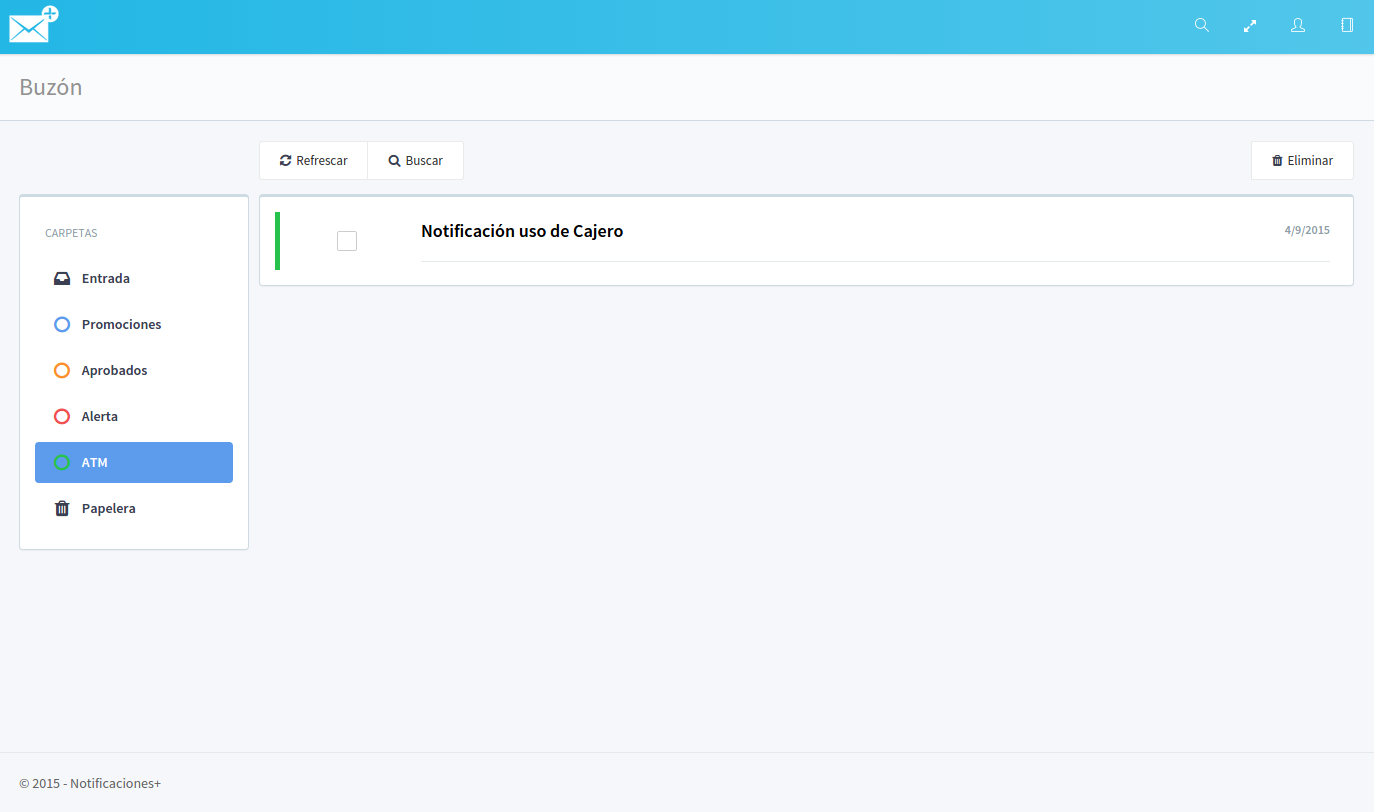
\includegraphics[width=11cm]{imagenes/Filtro4}} 
  % \quad
  \subfloat[Papelera]{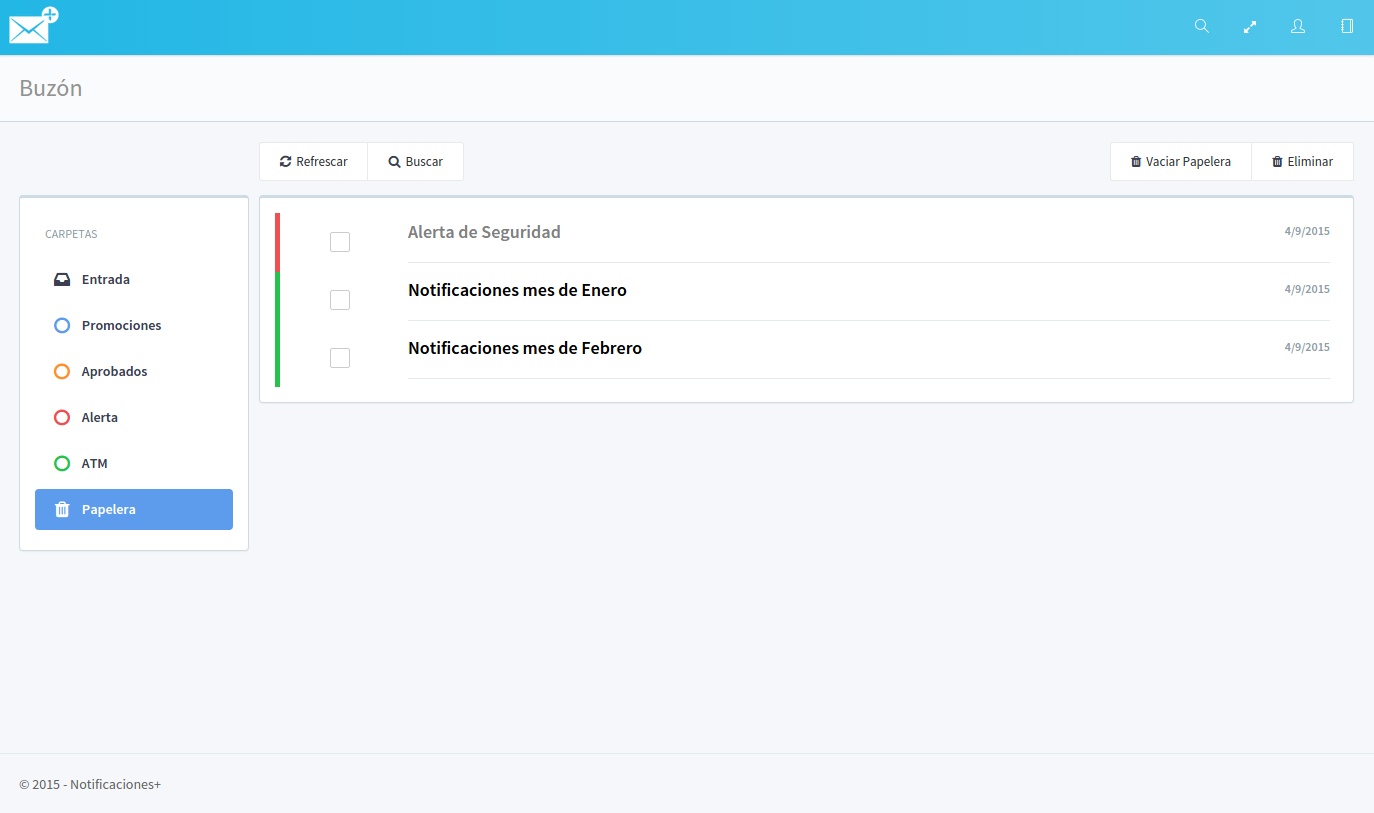
\includegraphics[width=11cm]{imagenes/Papelera}}
\caption{Pantalla de Buzón con botones de filtrado versión Web. Elaboración propia.}\label{fig:pantallaMultiWeb}
\end{figure}

% \begin{figure}[t]
% \centering
% \def\tabularxcolumn#1{m{#1}}
% \begin{tabularx}{\linewidth}{c}
% % 
%   \begin{tabular}{ccc}
%     \subfloat[Buzón de mensajes]{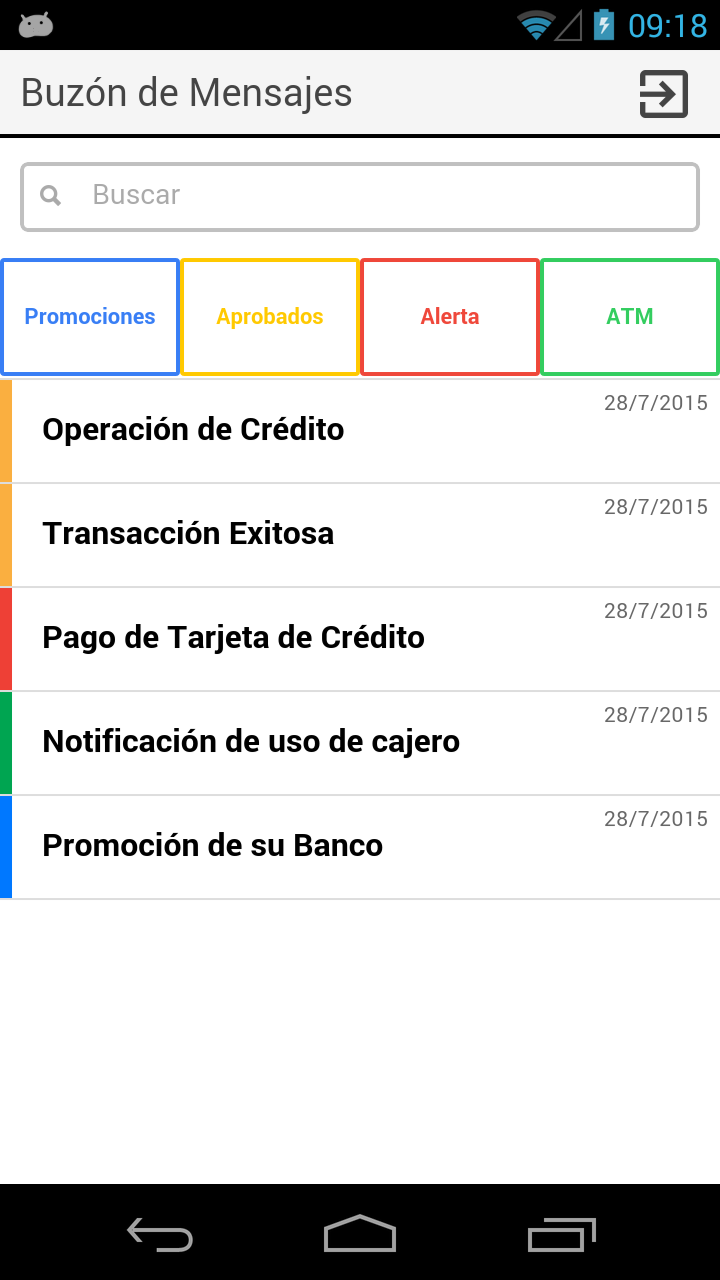
\includegraphics[width=3cm,type=png,ext=.png,read=.png,angle=0]{imagenes/pantalla5}} 
%     & \subfloat[Filtro Aprobados]{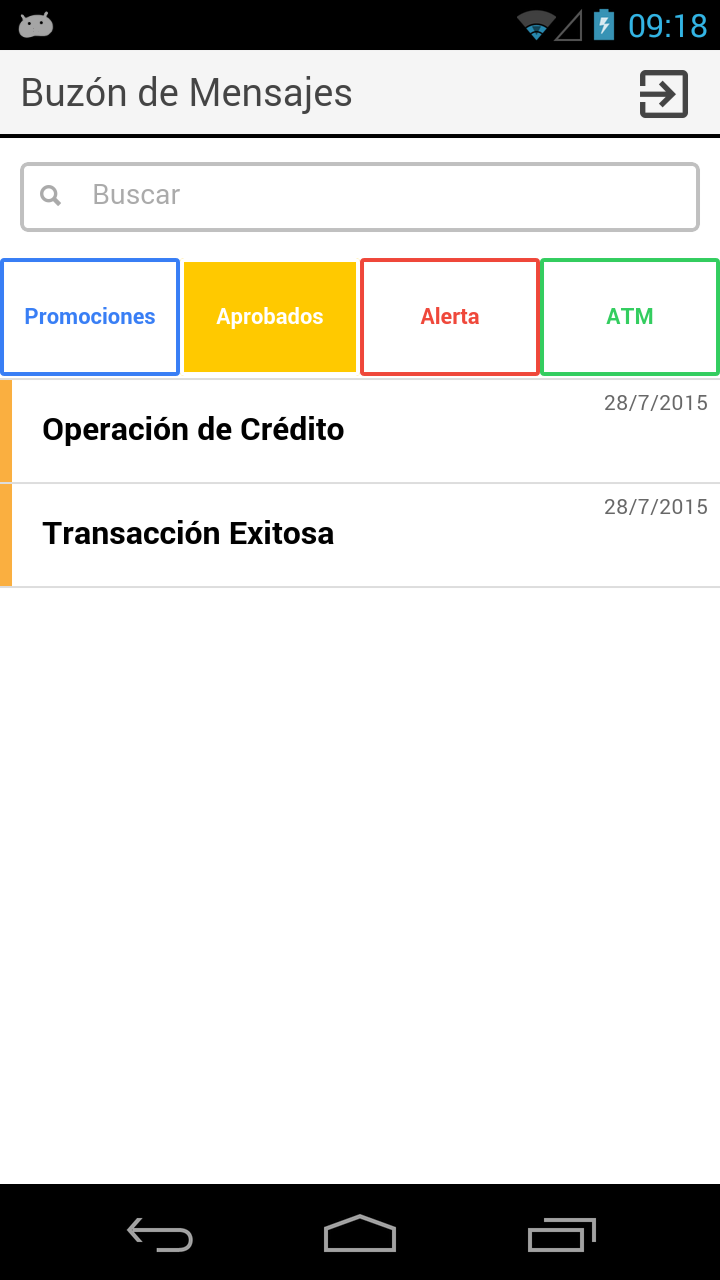
\includegraphics[width=3cm,type=png,ext=.png,read=.png,angle=0]{imagenes/pantalla6}}
%     & \subfloat[Filtro Promociones]{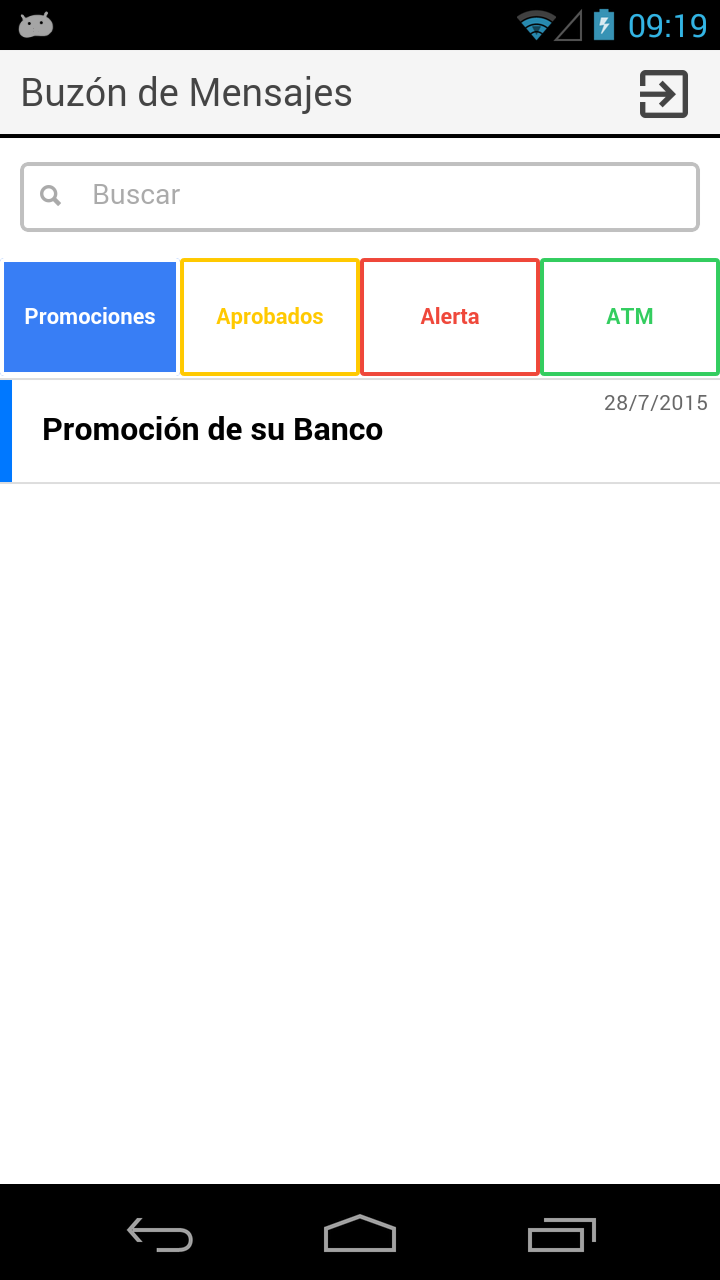
\includegraphics[width=3cm,type=png,ext=.png,read=.png,angle=0]{imagenes/pantalla7}}\\
%     \subfloat[Filtro Alerta]{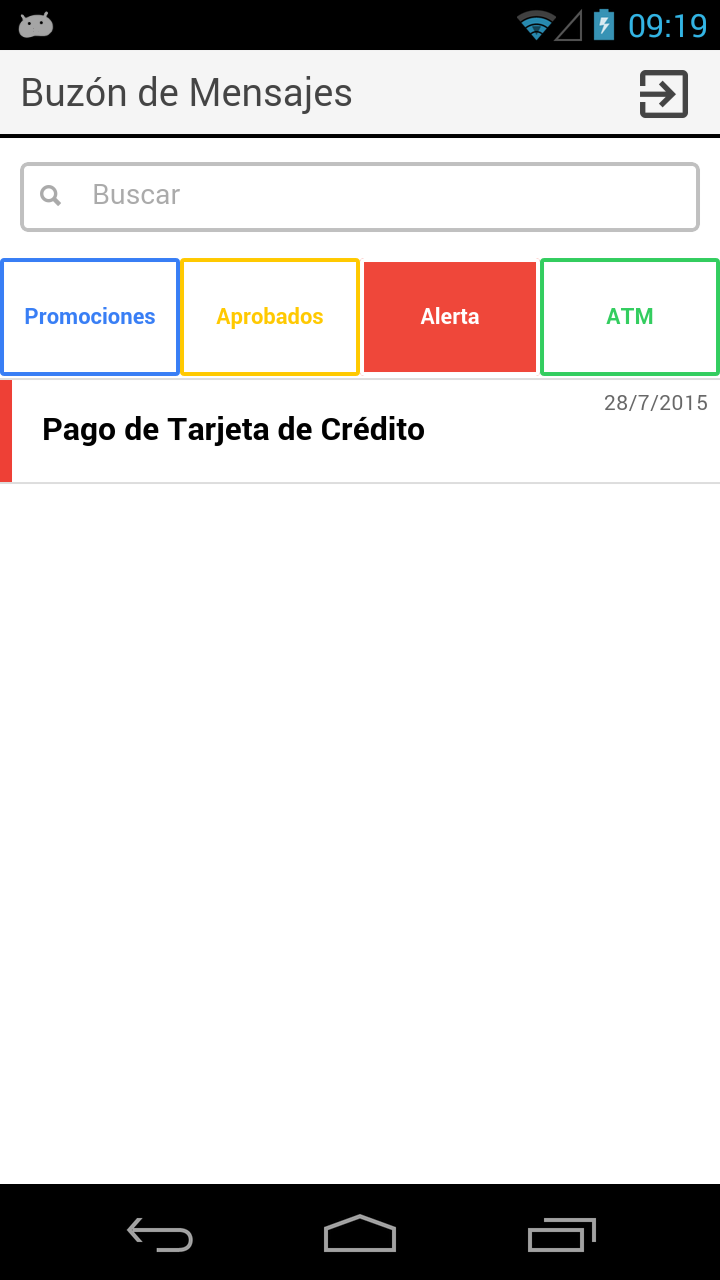
\includegraphics[width=3cm,type=png,ext=.png,read=.png,angle=0]{imagenes/pantalla8}}
%     & \subfloat[Filtro ATM]{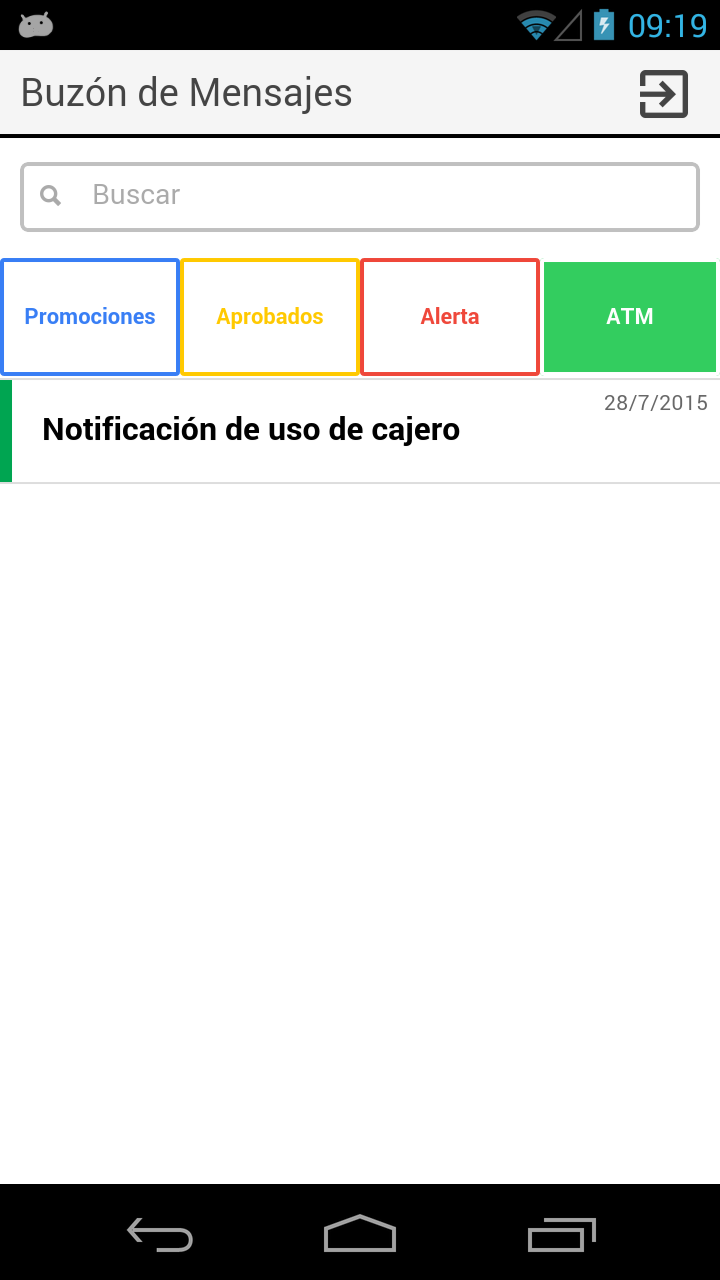
\includegraphics[width=3cm,type=png,ext=.png,read=.png,angle=0]{imagenes/pantalla9}} 
%     & \subfloat[Mensaje leído]{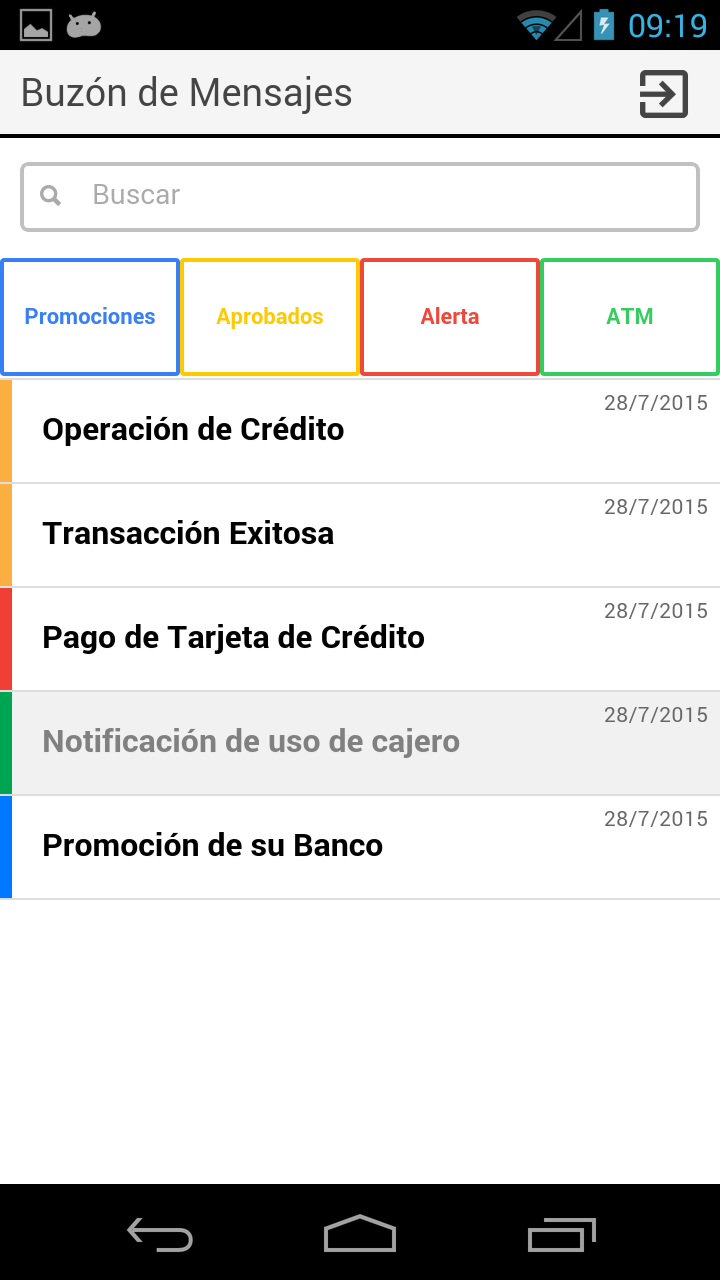
\includegraphics[width=3cm,type=png,ext=.png,read=.png,angle=0]{imagenes/pantalla10}}\\
%   \end{tabular}
% \end{tabularx}

% \caption{Pantalla de Buzón con botones de filtrado. Elaboración propia.}\label{fig:pantallaMulti}
% \end{figure}

Al deslizar un mensaje hacia la izquierda se muestra los botones de opcíon de compartir y eliminar. De seleccionarse eliminar se mostrará un menú de confirmación. El aspecto de los menús de confirmación y de las opciones para compartir dependen de la plataforma de la aplicación (iOS o Android). Ver la Figura ~\ref{fig:pantallaMulti2}.

\begin{figure}[htp]
\centering
  \subfloat[Opciones de mensaje]{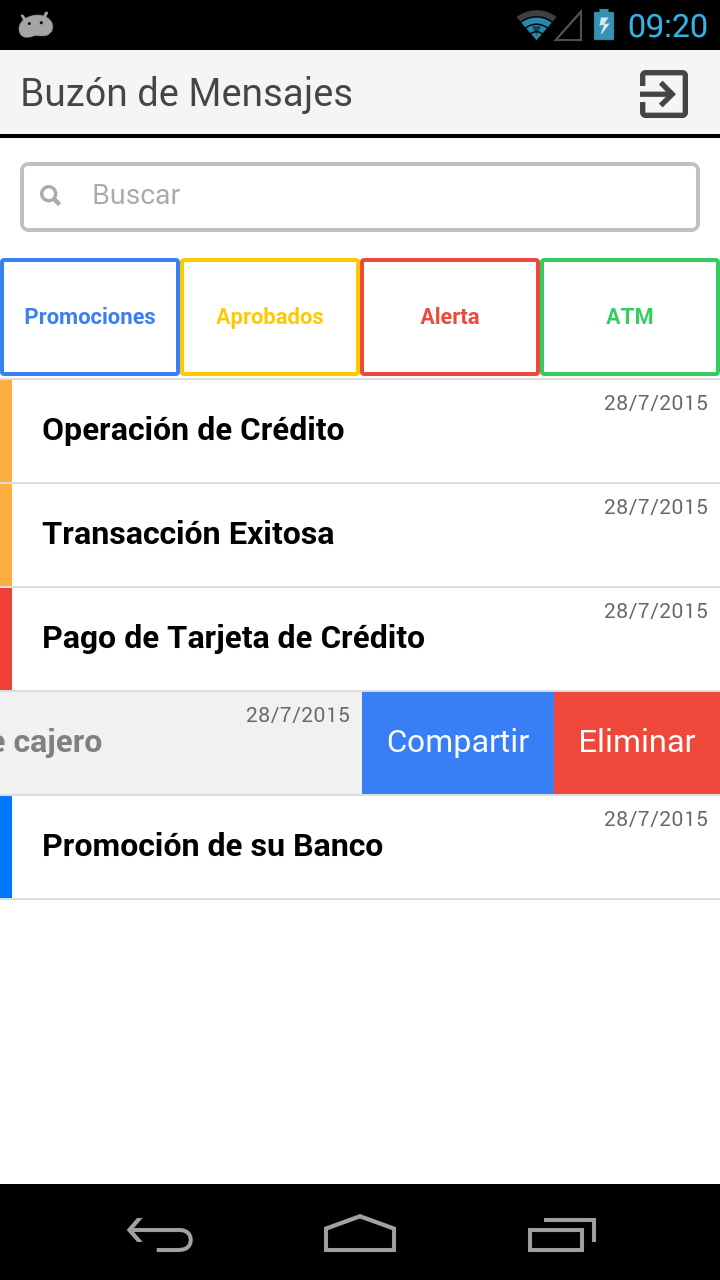
\includegraphics[width=3.5cm]{imagenes/pantalla11}} 
  \quad
  \subfloat[Confirmación de eliminar (Android)]{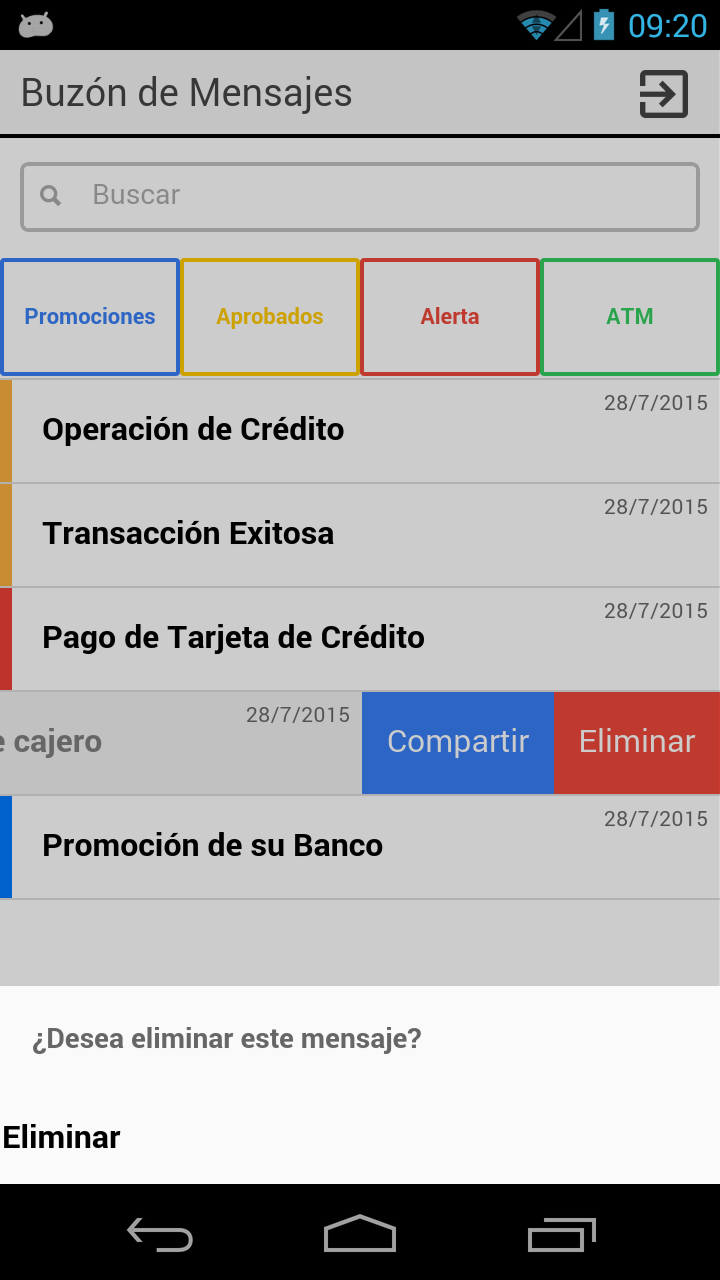
\includegraphics[width=3.5cm]{imagenes/pantalla12}}
  \quad
  \subfloat[Confirmación de eliminar (iOS)]{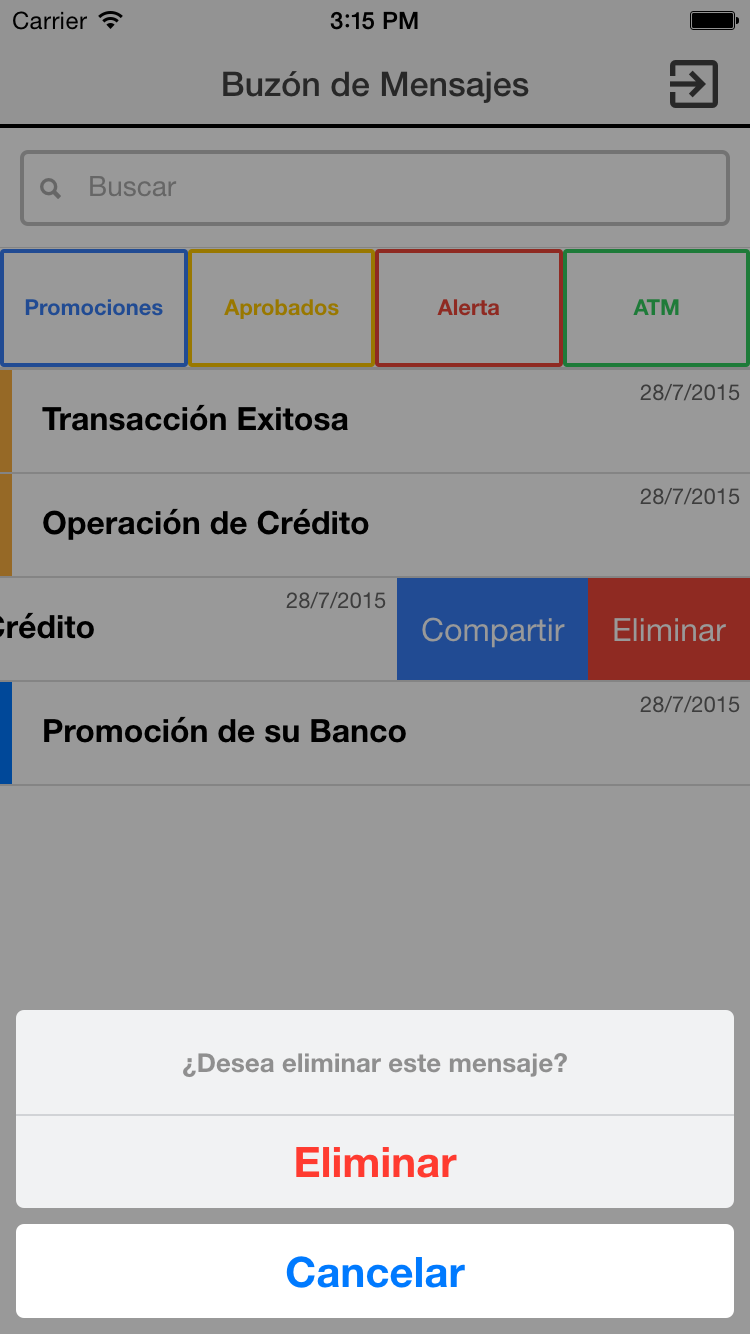
\includegraphics[width=3.5cm]{imagenes/iOSelim}}
\caption{Pantalla de Buzón con opciones de mensaje. Elaboración propia.}\label{fig:pantallaMulti2}
\end{figure}

% \begin{figure}[htp]
% \centering

% \subcaptionbox{Opciones de mensaje}{%
%   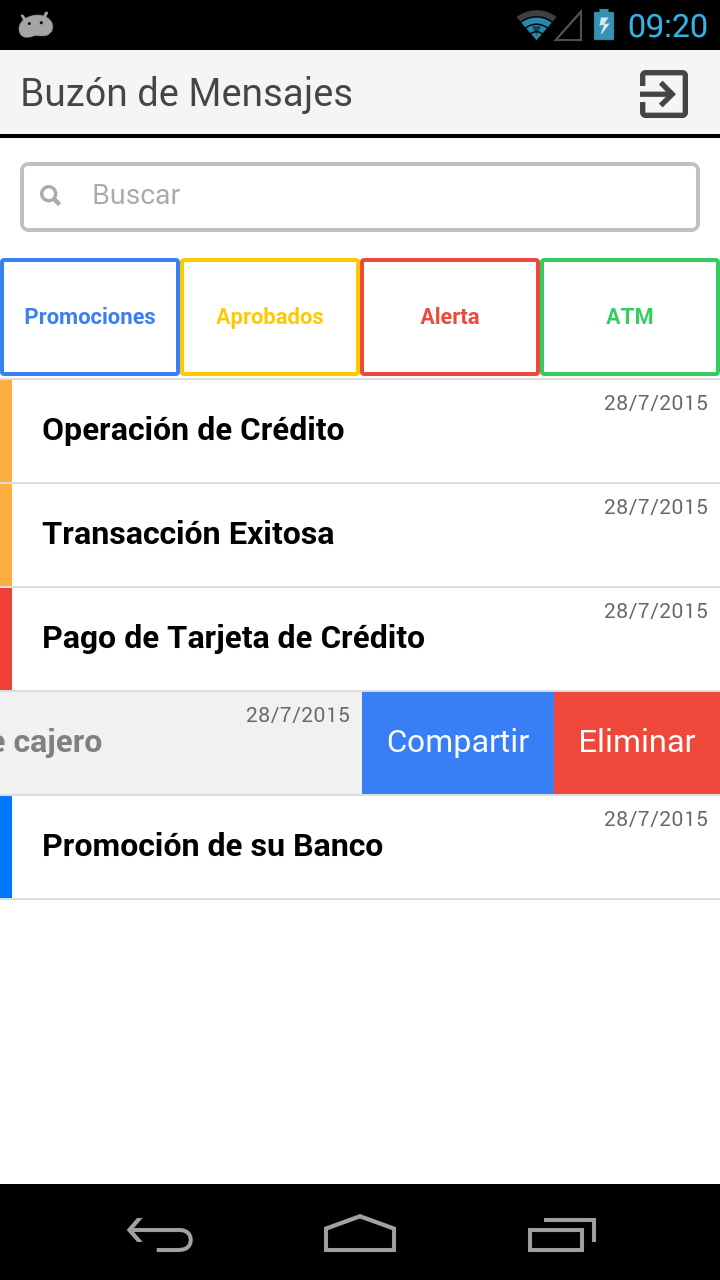
\includegraphics[width=3cm]{imagenes/pantalla11}%
% }\quad
% \subcaptionbox{Confirmación de eliminar (Android)}{%
%   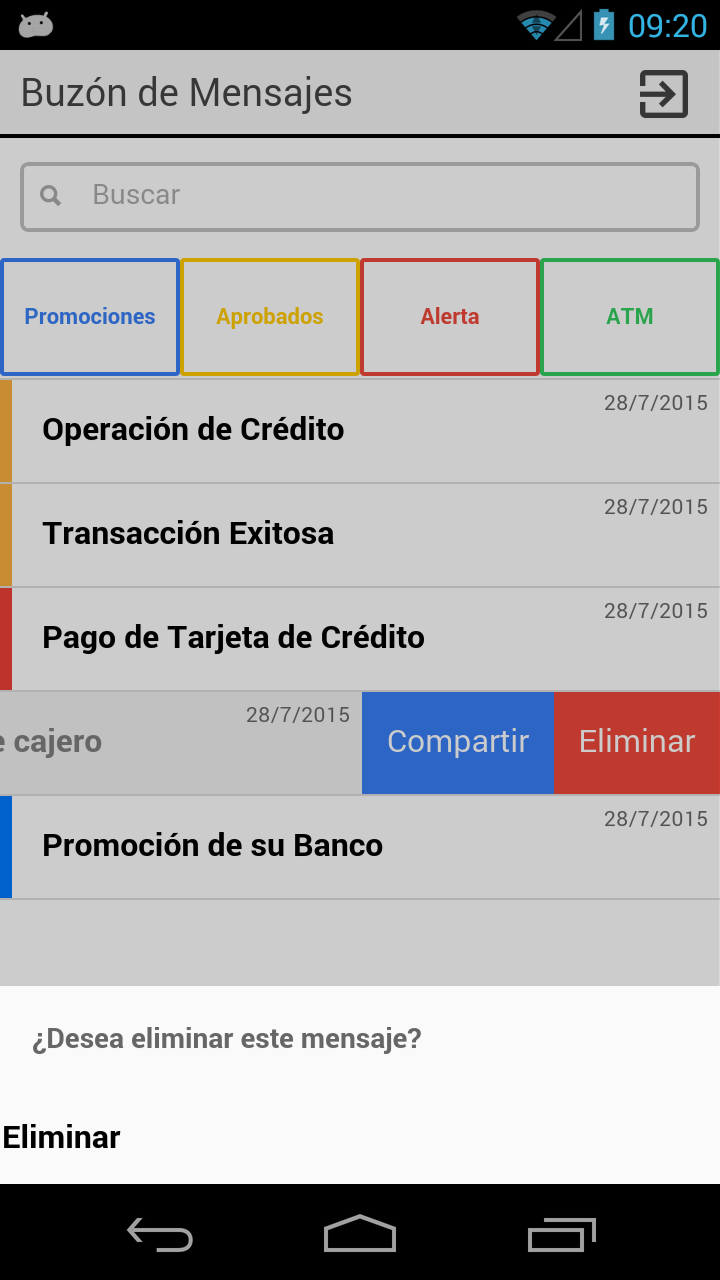
\includegraphics[width=3cm]{imagenes/pantalla12}%
% }\quad
% \subcaptionbox{Confirmación de eliminar (iOS)}{%
%   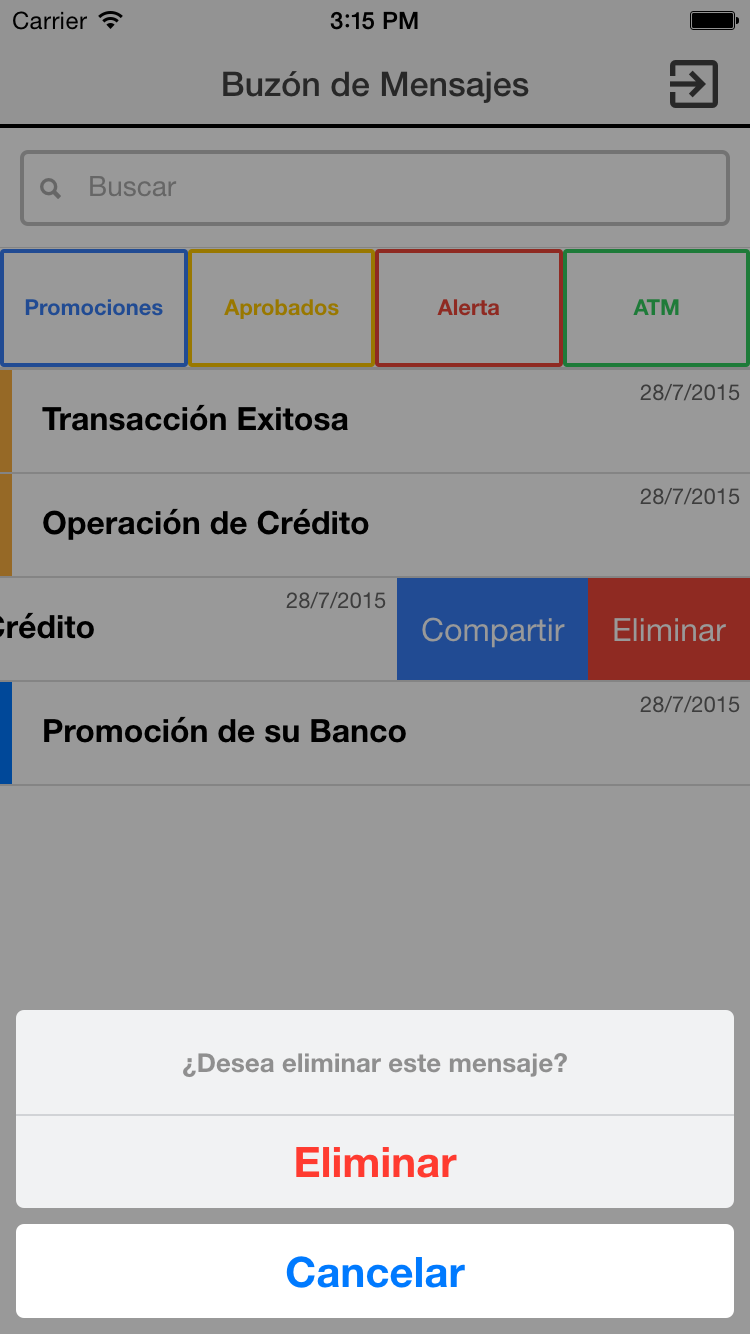
\includegraphics[width=3cm]{imagenes/iOSelim}%
% }

% \caption{Pantalla de Buzón con opciones de mensaje. Elaboración propia.}
% \label{fig:pantallaMulti2}

% \end{figure}

% \begin{figure}[t]
% \centering
% \def\tabularxcolumn#1{m{#1}}
% \begin{tabularx}{\linewidth}{c}
% %
%   \begin{tabular}{ccc}
%     \subfloat[Opciones de mensaje]{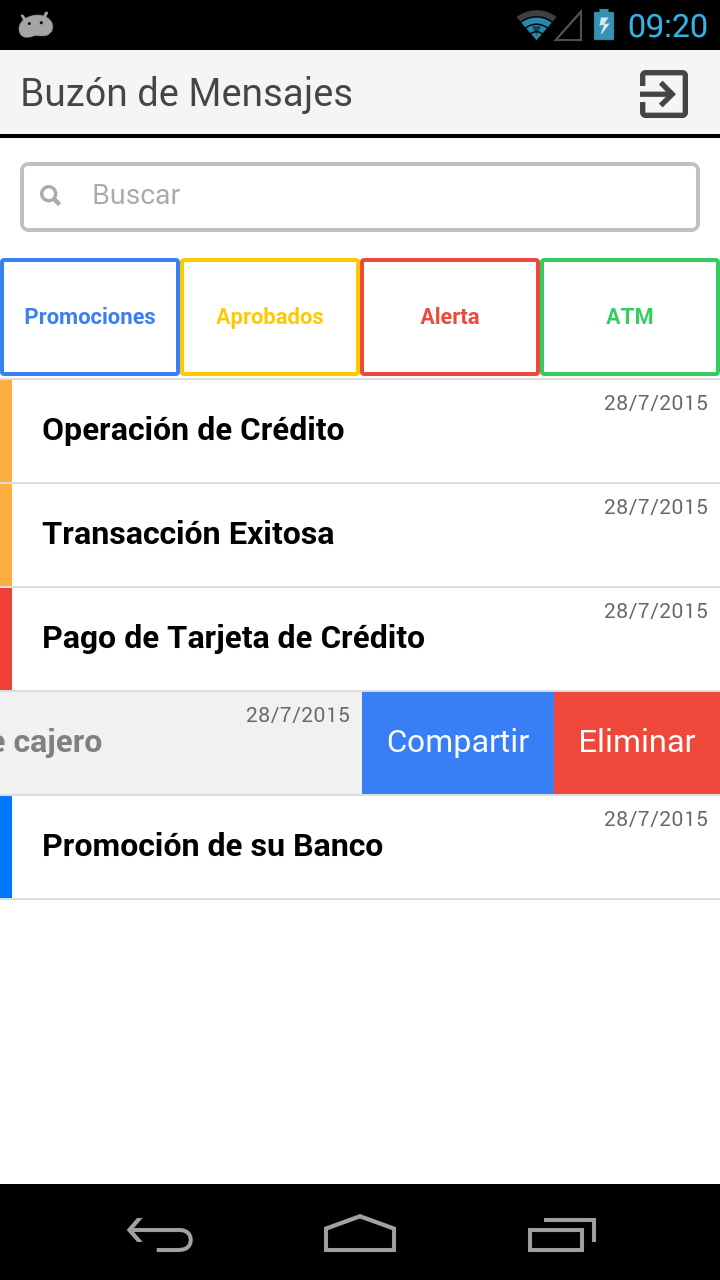
\includegraphics[width=3cm,type=png,ext=.png,read=.png,angle=0]{imagenes/pantalla11}} 
%     & \subfloat[Confirmación de eliminar (Android)]{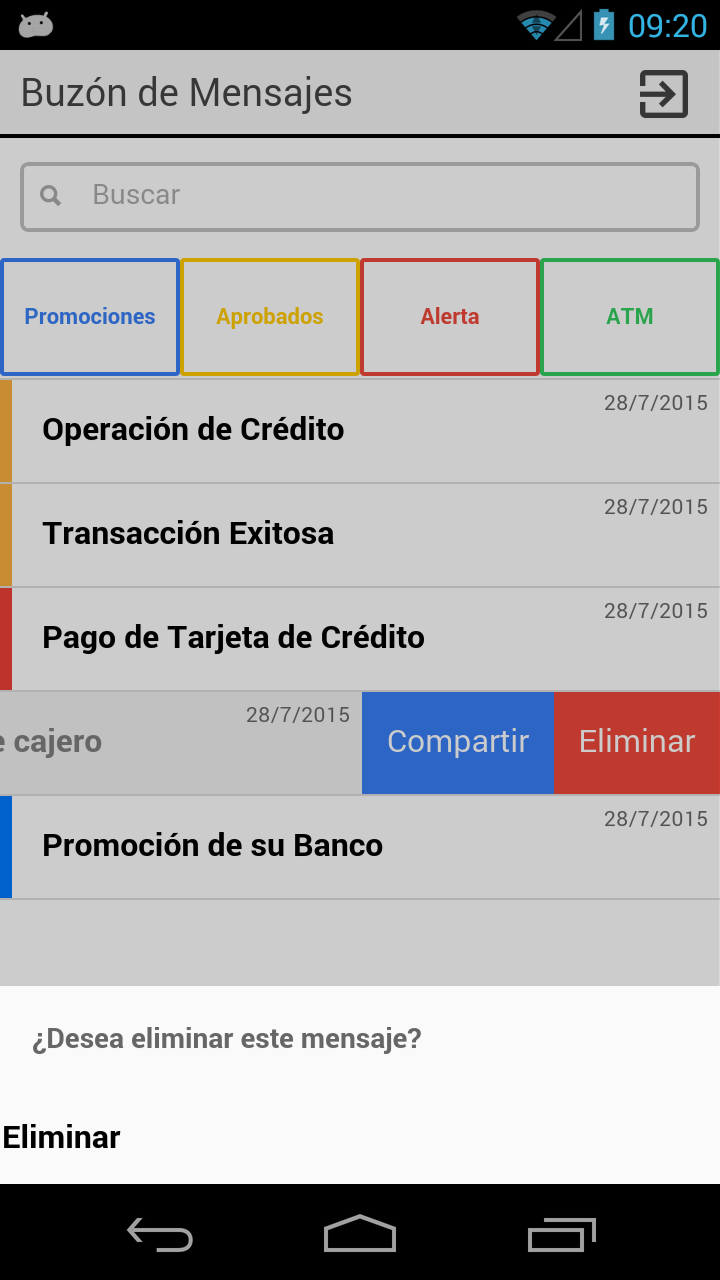
\includegraphics[width=3cm,type=png,ext=.png,read=.png,angle=0]{imagenes/pantalla12}}
%     & \subfloat[Confirmación de eliminar (iOS)]{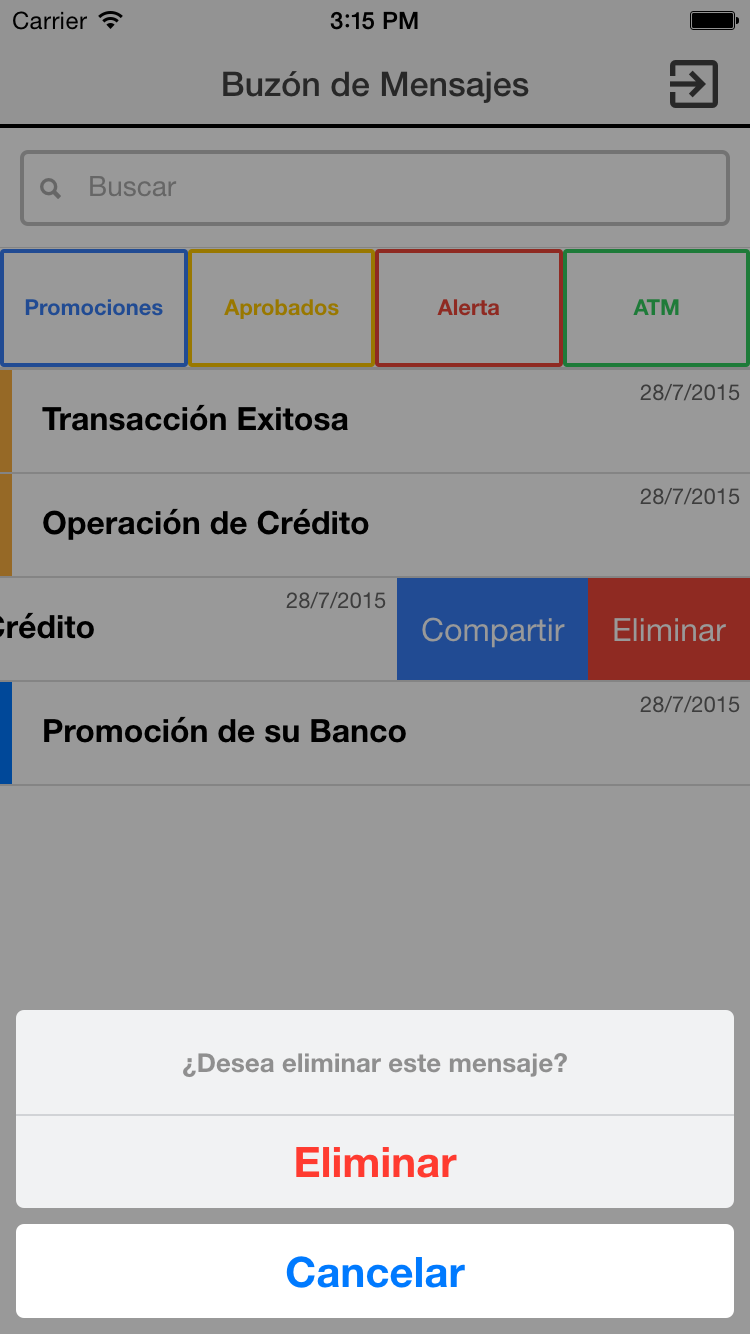
\includegraphics[width=3cm,type=png,ext=.png,read=.png,angle=0]{imagenes/iOSelim}}\\
%   \end{tabular}
% \end{tabularx}

% \caption{Pantalla de Buzón con opciones de mensaje. Elaboración propia.}\label{fig:pantallaMulti2}
% \end{figure}	

\section{Transición} \label{sect:Transicion}
La fase de transición no fue llevada a cabo debido a que el objetivo del proyecto fue, desde su concepción, la elaboración de un prototipo inicial 100\% funcional. Es por esto que tanto la aplicación web como la aplicación móvil de Notificaciones+ aún no ha entrado en una fase formal de transición a producción. Sin embargo, la plataforma Synergy Push (que provee los servicios de los que hace uso Notificaciones+) si se encuentra en producción y ya está siendo utilizada por bancos clientes de la empresa, así que la puesta en producción de Notificaciones+ dependería del momento en que la empresa quiera hacerlo.
